\documentclass[a4paper]{article}

% CJK support: prefer ctex, fallback to XeTeX native line breaking
\IfFileExists{ctex.sty}{
  \usepackage[fontset=fandol]{ctex}
}{
  % Fallback for minimal TeX installs (e.g. MacTeX Basic, TeX Live scheme-basic)
  % without ctex/xeCJK. Uses XeTeX's built-in CJK line breaking.
  \usepackage{fontspec}
  \XeTeXlinebreaklocale "zh"
  \XeTeXlinebreakskip = 0pt plus 1pt
  \IfFontExistsTF{Songti SC}{\setmainfont{Songti SC}}{%
    \IfFontExistsTF{Noto Serif CJK SC}{\setmainfont{Noto Serif CJK SC}}{}%
  }
  \IfFontExistsTF{Heiti SC}{\setsansfont{Heiti SC}}{%
    \IfFontExistsTF{Noto Sans CJK SC}{\setsansfont{Noto Sans CJK SC}}{}%
  }
}

% Basic packages
\usepackage{amsmath, amssymb}
\usepackage{graphicx}
\usepackage[margin=2.5cm]{geometry}
\emergencystretch=3em
\usepackage[most]{tcolorbox}
\usepackage{etoolbox}
\usepackage{listings}
\usepackage{hyperref}
\usepackage{booktabs}
\usepackage{array}
\usepackage{subcaption}
\usepackage{float}
\usepackage{tikz}
\IfFileExists{pgfplots.sty}{
    \usepackage{pgfplots}
    \pgfplotsset{compat=1.18}
}{}

% ===== Highlight boxes =====
\newtcolorbox{knowledgebox}[1]{
    enhanced, colback=blue!5!white, colframe=blue!75!black, colbacktitle=blue!75!black,
    coltitle=white, fonttitle=\bfseries, title={#1}, attach boxed title to top left={yshift=-2mm, xshift=2mm},
    boxrule=1pt, sharp corners
}

\newtcolorbox{importantbox}[1]{
    enhanced, colback=yellow!10!white, colframe=yellow!80!black, colbacktitle=yellow!80!black,
    coltitle=black, fonttitle=\bfseries, title={#1}, sharp corners
}

\newtcolorbox{warningbox}[1]{
    enhanced, colback=red!5!white, colframe=red!75!black, colbacktitle=red!75!black,
    coltitle=white, fonttitle=\bfseries, title={#1}, sharp corners
}

\newtcolorbox{practicebox}[1]{
    enhanced, colback=black!3!white, colframe=black!75, colbacktitle=black!75,
    coltitle=white, fonttitle=\bfseries, title={#1}, sharp corners
}

% ===== Code listings =====
\lstset{
    basicstyle=\ttfamily\small,
    keywordstyle=\color{blue},
    stringstyle=\color{red!60!black},
    commentstyle=\color{green!60!black},
    breaklines=true,
    frame=single,
    numbers=left,
    numberstyle=\tiny\color{gray},
    captionpos=b,
    extendedchars=false
}

% ===== Figure provenance and unit macros =====
% \vtag goes inside \caption{...}; \srcnote{MM:SS--MM:SS} follows the figure environment.
\newcommand{\vtag}{\protect\footnotemark}
\newcommand{\srcnote}[1]{\footnotetext{视频画面时间区间：#1。若为裁剪图，时间区间仍对应原视频画面。}}
% Units work in text and math mode; never hand-write $^\circ$ or \AA inside \mathrm.
\newcommand{\degC}{\ensuremath{^{\circ}\mathrm{C}}}
\newcommand{\um}{\ensuremath{\mu\mathrm{m}}}
\newcommand{\nm}{\ensuremath{\mathrm{nm}}}
\newcommand{\angstrom}{\ensuremath{\text{\AA}}}

% ===== Front-page metadata =====
% Fill these in when generating notes.
\newcommand{\notetitle}{课程概览与 Shell 入门}
\newcommand{\notesubtitle}{MIT Missing Semester 2026 · 第 1 讲：终端、命令、路径、常用程序与 Shell 脚本}
\newcommand{\noteauthors}{根据 MIT Missing Semester 2026 课堂录像整理（Jon 主讲）}
\newcommand{\notedate}{2026年1月12日（课堂）}
\newcommand{\videochannel}{Missing Semester（YouTube）}
\newcommand{\videopublishdate}{2026年}
\newcommand{\videoduration}{1小时14分43秒}
\newcommand{\videourl}{https://www.youtube.com/watch?v=MSgoeuMqUmU}
\newcommand{\videocoverpath}{cover.jpg}

\setlength{\emergencystretch}{3em}
\begin{document}

% ===== Title page =====
\begin{titlepage}
\centering
{\Large 课程笔记\par}
\vspace{1.2cm}
{\huge\bfseries \notetitle\par}
\ifdefempty{\notesubtitle}{}{
\vspace{0.3cm}
{\large \notesubtitle\par}
}
\vspace{0.5cm}
{\large \noteauthors\par}
\vspace{0.3cm}
{\large \notedate\par}
\vspace{1.0cm}

\ifdefempty{\videocoverpath}{
{\small 请在生成笔记时填入视频封面图的本地路径。\par}
}{
\includegraphics[width=0.82\textwidth,height=0.40\textheight,keepaspectratio]{\videocoverpath}\par
}

\vfill
\begin{tcolorbox}[width=0.9\textwidth, colback=black!2!white, colframe=black!60, sharp corners]
\textbf{视频作者/频道}：\videochannel\par
\textbf{发布日期}：\videopublishdate\par
\textbf{视频时长}：\videoduration\par
\textbf{视频链接}：
\ifdefempty{\videourl}{
未填写
}{
\href{\videourl}{\nolinkurl{\videourl}}
}
\end{tcolorbox}
\end{titlepage}

\tableofcontents
\newpage

%% --- 正文内容开始 --- %%

\section{这一讲讲什么}

这是 MIT Missing Semester 2026 的第一讲，主题是课程概览与 Shell 入门。开场时三位讲者 Anish、Jon 和 Jose 一起站在台上介绍课程，之后由 Jon 讲授 Shell 部分。

\noindent\begin{minipage}{\textwidth}
\begin{figure}[H]
\centering
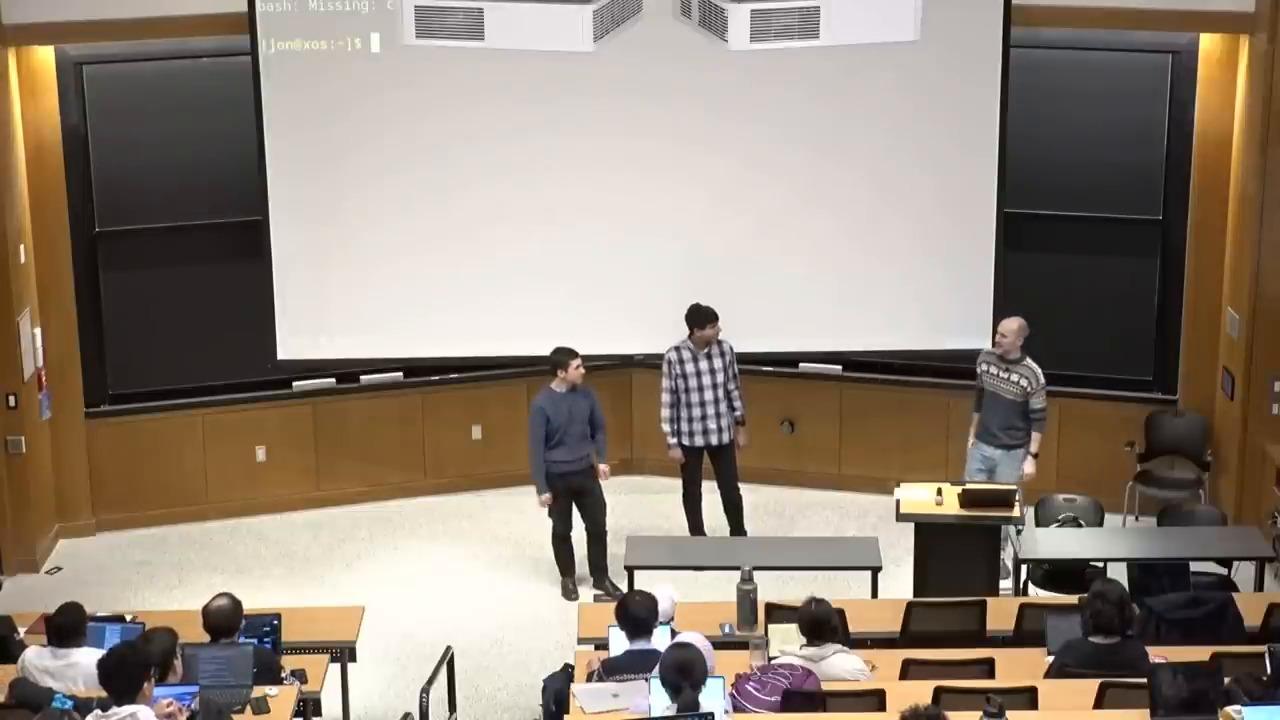
\includegraphics[width=0.92\textwidth]{figures/fig_01_room.jpg}
\caption{第一讲开场：三位讲者在教室前介绍课程\vtag}
\end{figure}
\srcnote{00:02:00--00:02:15}
\end{minipage}


\subsection{为什么开这门课}

讲者介绍，这门课最早在 2019 年开设，2020 年又开了一次，此后三人都去做别的事了。但有足够多的人觉得这门课有用，而且自上次以来变化的东西也足够多，于是决定再开一轮。三人都是在 MIT 读博期间开这门课的校友。他们在 MIT 上了很多课，都经历过同一种痛苦：课程默认你已经会 Git、会用编辑器、会在终端里四处走动，甚至默认你知道终端是什么。讲者认为，掌握这些东西是一种“超能力”。

另一位讲者补充了灵感来源：读研期间他们当过很多课的助教，经常在答疑时间里教学生的并不是课程本身的内容，而是怎样用 Shell、怎样最有效地使用文本编辑器这类事情。于是他们想把这些主题单独“提取”出来，专门开一门课讲，好让学生在其他课上专注于课程本身。还有一类问题，比如“这个任务怎样自动化”，学生甚至不会想到去问，因为他们不知道这是可能的。

第三位讲者说，这在一定程度上是“未知的未知”：很多聪明的程序员早就遇到过同样的烦恼，也早已解决了它们，但这些解法不会在编译原理课或算法课上讲，所以你可能根本不知道它们存在。

\begin{importantbox}{这门课的定位}
讲者说，由于时间有限，课程不可能深入讲解每一个工具和技巧。很大程度上，这门课像是一种“暴露疗法”：向你展示什么是可能的、有哪些工具值得知道，但未必详细讲它们怎样工作或该怎样用。目的是让你知道这些工具，然后自己去阅读、自己去实验。每一讲都附有习题，讲义里也有课上没讲到的内容。
\end{importantbox}

\subsection{课程安排}

讲者介绍，接下来两周每天下午 $1$:$30$ 到 $2$:$30$ 上课，周五例外，因为教室那时被占用，周五改为 $3$ 点开始；下周一放假。讲者说最后一个周五（不是这周五，而是下周五）的课会完全用来答疑，希望大家在前两周积累一些“这到底怎么工作的”“能不能多讲讲这个”之类的问题。课后有问题，可以在网站上链接的 Discord 频道里提问，那是开源大学（OSSU）社区的一个频道，也可以发邮件给讲者；讲者希望把回答记录下来，让其他有同样问题的人也能受益。

\begin{knowledgebox}{2026 年的九讲}
根据课程网站，2026 年的九讲依次是：课程概览与 Shell 入门、命令行环境、开发环境与工具、调试与性能分析、版本控制与 Git、打包与发布代码、智能体编程（agentic coding）、代码之外，以及代码质量。各讲基本独立，但后面的课会假定你熟悉前面的内容。
\end{knowledgebox}

\section{Shell 是什么}

\subsection{为什么要用文本界面}

讲者说，计算机有很多种交互界面：大家熟悉的图形用户界面（GUI），移动鼠标、点击按钮，设计得好的 GUI 很好用；近来还有智能体（agentic）界面、语音等。但它们有局限：在 GUI 里你只能做程序里预先编好的事；想把两个做相关工作的程序结合起来，往往很难，需要 A 厂商的软件 A 和 B 厂商的软件 B 专门实现互通。有时你就是想下沉一层，到一个可以随意写命令、把命令串起来的地方，这就是 Shell。

\subsection{终端与 Shell}

\noindent\begin{minipage}{\textwidth}
\begin{figure}[H]
\centering
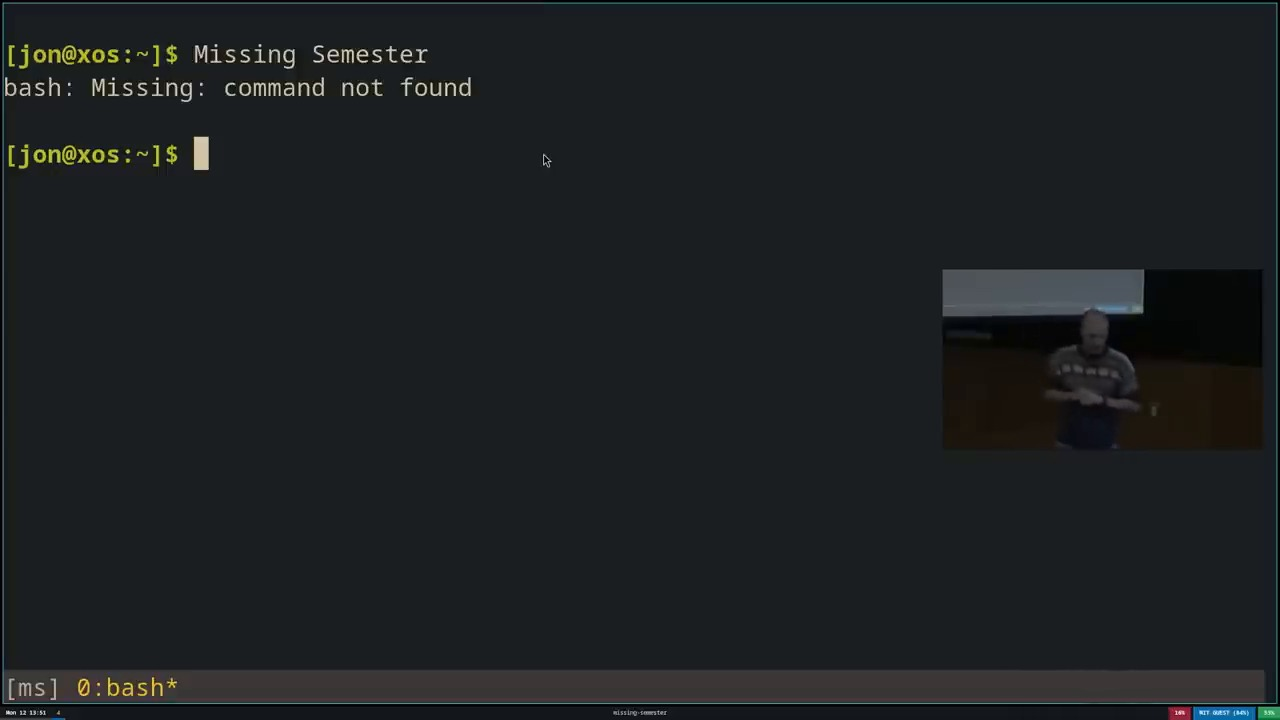
\includegraphics[width=0.92\textwidth]{figures/fig_02_prompt.jpg}
\caption{终端里的 bash 提示符，显示用户名、主机名和当前目录\vtag}
\end{figure}
\srcnote{00:14:30--00:14:45}
\end{minipage}


Shell 运行在终端（terminal）之中。讲者说可以把终端想成包在 Shell 外面的那个 GUI 窗口：屏幕上带边框的这个东西就是他的终端，里面没有其他界面元素；有的终端有，他的没有。终端负责的是移动、选择文本这类事，有意思的部分几乎都发生在 Shell 里。大多数电脑都自带终端：Linux 上通常按 Ctrl+Alt+T，也可以在应用启动器里搜索 terminal；macOS 和 Windows 上也有类似的办法。

最常用的 Shell 是 Bourne Again SHell，即 bash，Linux 上打开终端通常得到的就是它。macOS 过去也默认用 bash，如今默认是 zsh，一些 Linux 发行版也是。zsh 与 bash 兼容，bash 里合法的东西在 zsh 里通常也合法，并且 zsh 有许多易用性改进。讲者说三位讲者自己用的 Shell 各不相同，大家以后也可以探索自己的选择，但本课程的内容都以 bash，进而也以 zsh 为准。Windows 上得到的不是兼容 bash 的提示符，而是 batch（B-A-T-C-H）或较新的 PowerShell，概念相似，但语法不同。

\subsection{为什么值得学}

讲者给出几点理由：一旦习惯了，Shell 通常比到处点击快得多，敲很少的键就能做很多事，而在 GUI 里任务越复杂越费力；更重要的是 Shell 可以自动化。讲者说 Shell 本质上是一门编程语言，提示符就像是一个你可以往里写东西的文件的开头，你写下的就是一个会被执行的 bash 程序。会用 Shell 还便于参与开源社区：几乎任何开源工具的构建、安装和运行说明都在 Shell 里完成；越来越多的“我的电脑上怎样做某事”的答案也是“打开终端，输入这个”。知道这条命令大致做了什么，总比盲目地从 Stack Overflow 复制粘贴、心想“应该没问题吧”要好。

\subsection{读懂提示符}

提示符是 Shell 的主要界面。讲者解释了他的提示符：开头说明用户名是 \texttt{jon}，所在机器的主机名是 \texttt{xos}；冒号是分隔符，就像 @ 一样；波浪线 \textasciitilde{} 之后是当前在文件系统中的位置，而波浪线本身是主目录的简写，所以他现在位于主目录；最后的美元符号表示他是普通用户而不是 root。他在提示符里输入 \texttt{Missing Semester}，Shell 回答 \texttt{Missing: command not found}，因为第一个词被当作了程序名。

\begin{knowledgebox}{终端、Shell 与提示符}
讲义作者整理三个容易混淆的名词：终端（终端模拟器）是显示文本、接收键盘输入的窗口程序；Shell 是在终端里运行、解释并执行命令的程序，例如 bash、zsh；提示符是 Shell 打印出来、等待你输入命令的那一行。换一个终端不会改变命令的语法，换一个 Shell 才会。
\end{knowledgebox}

\section{命令与参数}

\subsection{运行程序与传递参数}

\noindent\begin{minipage}{\textwidth}
\begin{figure}[H]
\centering
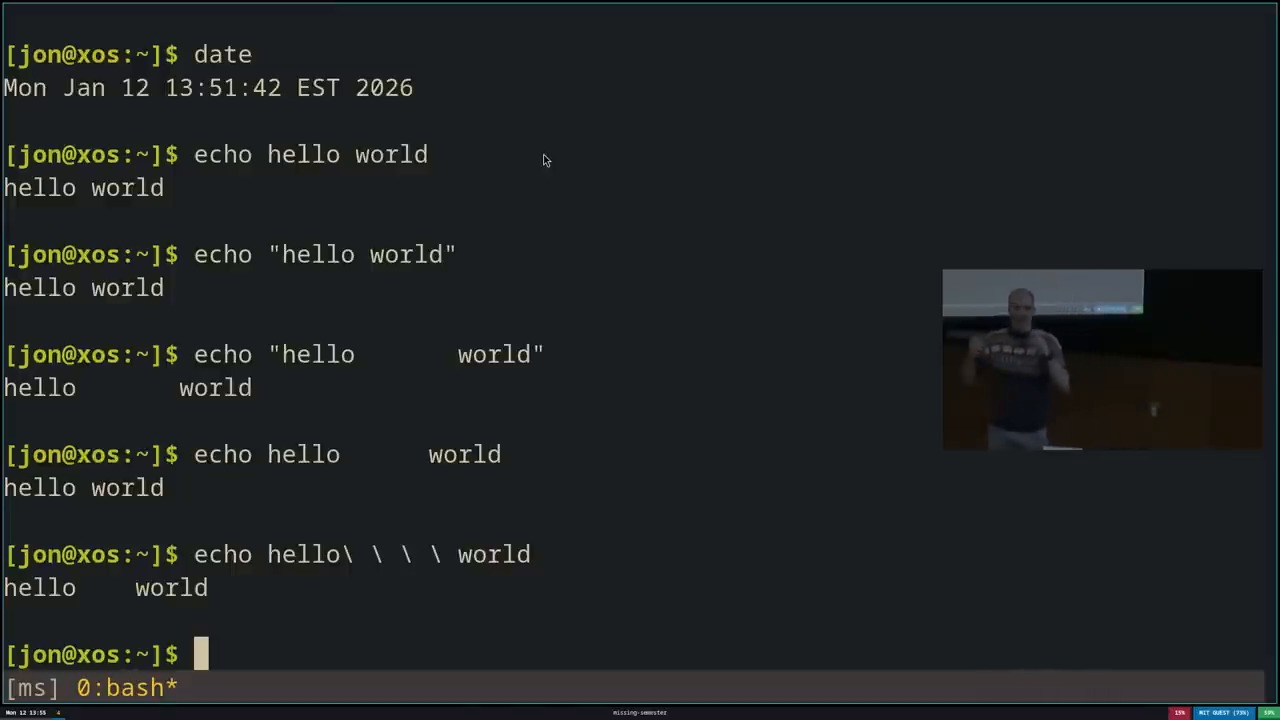
\includegraphics[width=0.92\textwidth]{figures/fig_03_echo_args.jpg}
\caption{\texttt{date} 与 \texttt{echo} 的运行结果：参数按空白切分\vtag}
\end{figure}
\srcnote{00:18:30--00:18:45}
\end{minipage}


在提示符里可以输入想执行的命令。最简单的命令就是一个程序名，例如 \texttt{date}，不出意外，它把当前日期打印到终端，然后你回到提示符，可以继续输入。命令也可以带参数，参数是跟在程序名后面的东西。例如 \texttt{echo} 会把它的参数打印出来。

讲者解释 Shell 怎样解析一条命令：拿到用户输入的文本，在空白处切分，每个以空白分隔的词就是一个参数，第一个词是要执行的程序。如果想要一个包含空白的参数，可以像大多数编程语言那样用引号。由于 \texttt{echo} 默认用单个空格连接它的各个参数打印出来，\texttt{echo hello world} 和 \texttt{echo "hello world"} 输出一样；但 \texttt{echo "hello      world"} 会保留中间的多个空格，因为它只是一个参数，而不加引号时多余的空格就消失了。

\subsection{引号与转义}

\noindent\begin{minipage}{\textwidth}
\begin{figure}[H]
\centering
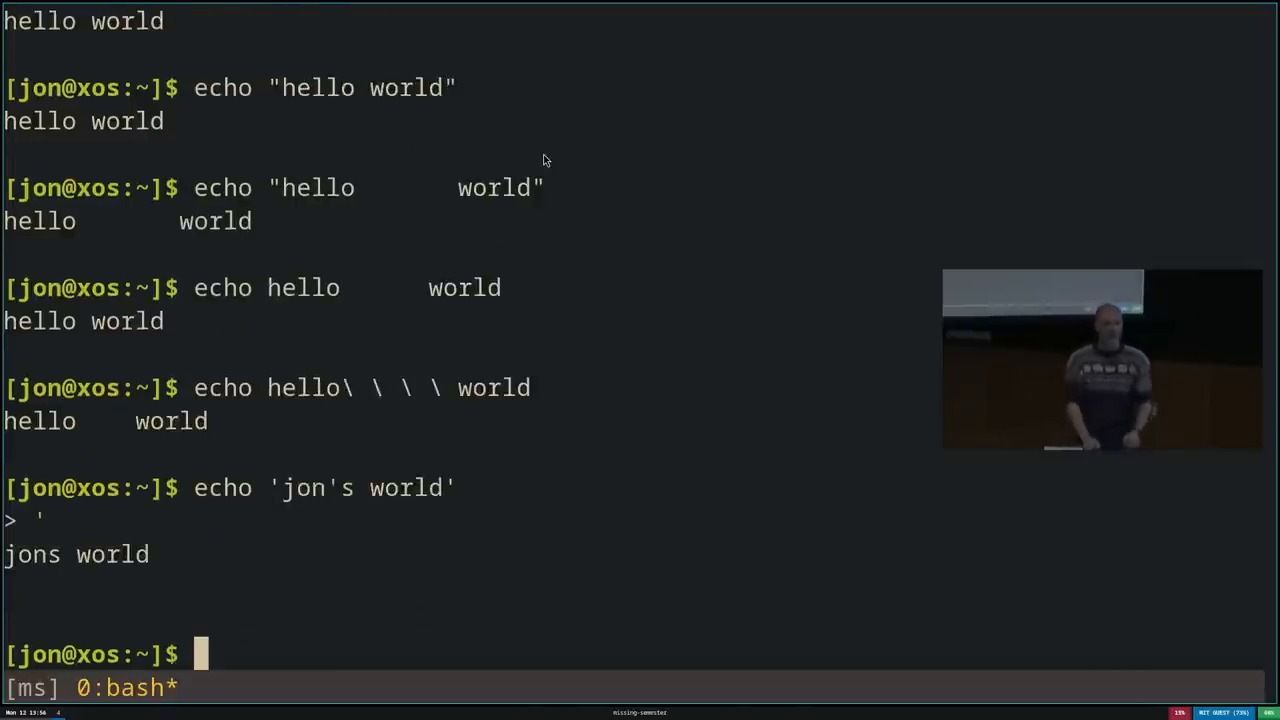
\includegraphics[width=0.92\textwidth]{figures/fig_04_escape.jpg}
\caption{用反斜杠转义空格，以及用双引号包住含单引号的字符串\vtag}
\end{figure}
\srcnote{00:20:00--00:20:15}
\end{minipage}


讲者说，自己写命令行时会经常遇到参数解析的问题，把引号写对有时相当烦人。有同学问为什么这些程序没有 \texttt{.java}、\texttt{.py} 之类的扩展名：讲者说很多都是安装在系统里的预编译程序，后面会讲它们在哪里；在 Python 里用 \texttt{sys.argv} 拿到的参数列表，正是从这里来的。

更复杂的情况下会遇到引号问题，比如路径里的文件名含有单引号，这时要么用双引号包住整个字符串，要么转义。转义就是在字符前加反斜杠，可以对多个字符分别转义。讲者解释，反斜杠是转义字符，意思是“别把下一个字符当作特殊字符”；在参数解析中，反斜杠加空格表示一个字面上的空格，不在这里切分。

他演示了 \texttt{echo jon's world}：Shell 认为单引号开始了一个字符串，却找不到结束的单引号，于是进入续行提示符，等待更多输入。可以写成 \texttt{echo jon\textbackslash's world}，或者用双引号把整个字符串包起来，就得到预期的输出。

\begin{warningbox}{单引号与双引号的区别}
讲义作者补充：在单引号内，所有字符都按字面处理，连 \texttt{\$} 和反斜杠也不例外，所以单引号里无法再放单引号；在双引号内，\texttt{\$var}、\texttt{\$(...)} 等仍会被展开。需要原样保留美元符号时用单引号，需要插入变量值时用双引号。
\end{warningbox}

\subsection{手册与帮助}

\noindent\begin{minipage}{\textwidth}
\begin{figure}[H]
\centering
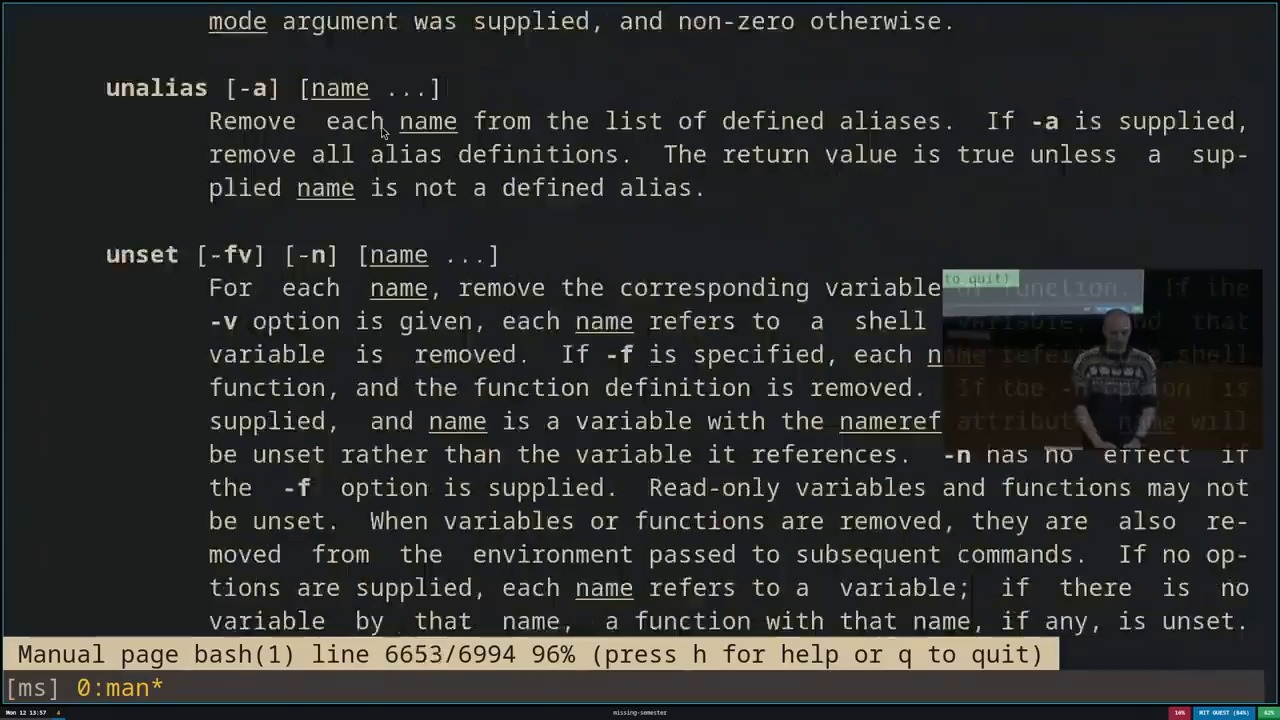
\includegraphics[width=0.92\textwidth]{figures/fig_05_man.jpg}
\caption{\texttt{man bash} 打开的手册页内容非常详尽\vtag}
\end{figure}
\srcnote{00:21:00--00:21:15}
\end{minipage}


Shell 里最有用的程序之一是 \texttt{man}，是 manual（手册）的缩写。给它另一个程序的名字，它会解释怎样使用那个程序，例如 \texttt{man echo}。bash 的手册页非常详尽，有错误报告、作者、文件、受限模式等等，解释了 bash 里你可能想做的各种事。讲者说你会经常用 \texttt{man} 来了解手头的命令能做什么。通常还可以给程序传 \texttt{-{}-help} 参数得到一个简短版本，例如 \texttt{date -{}-help} 打印出 \texttt{date} 的帮助文字，一般比手册页短一些。

\begin{knowledgebox}{更易读的帮助}
讲义作者补充：课程讲义推荐了 \texttt{tldr} 这类工具，它为常用命令给出简短的示例，比完整手册更适合快速上手；在 \texttt{man} 里可以按 \texttt{/} 搜索关键字，按 \texttt{q} 退出。
\end{knowledgebox}

\subsection{本章小结}

一条命令就是用空白分隔的一串词，第一个是程序，其余是参数；引号和反斜杠控制在哪里切分；\texttt{man} 和 \texttt{-{}-help} 告诉你一个程序能做什么。接下来要回答的问题是：Shell 在哪里，以及怎样在文件系统里移动。

\section{在文件系统中移动}

\subsection{绝对路径}

\noindent\begin{minipage}{\textwidth}
\begin{figure}[H]
\centering
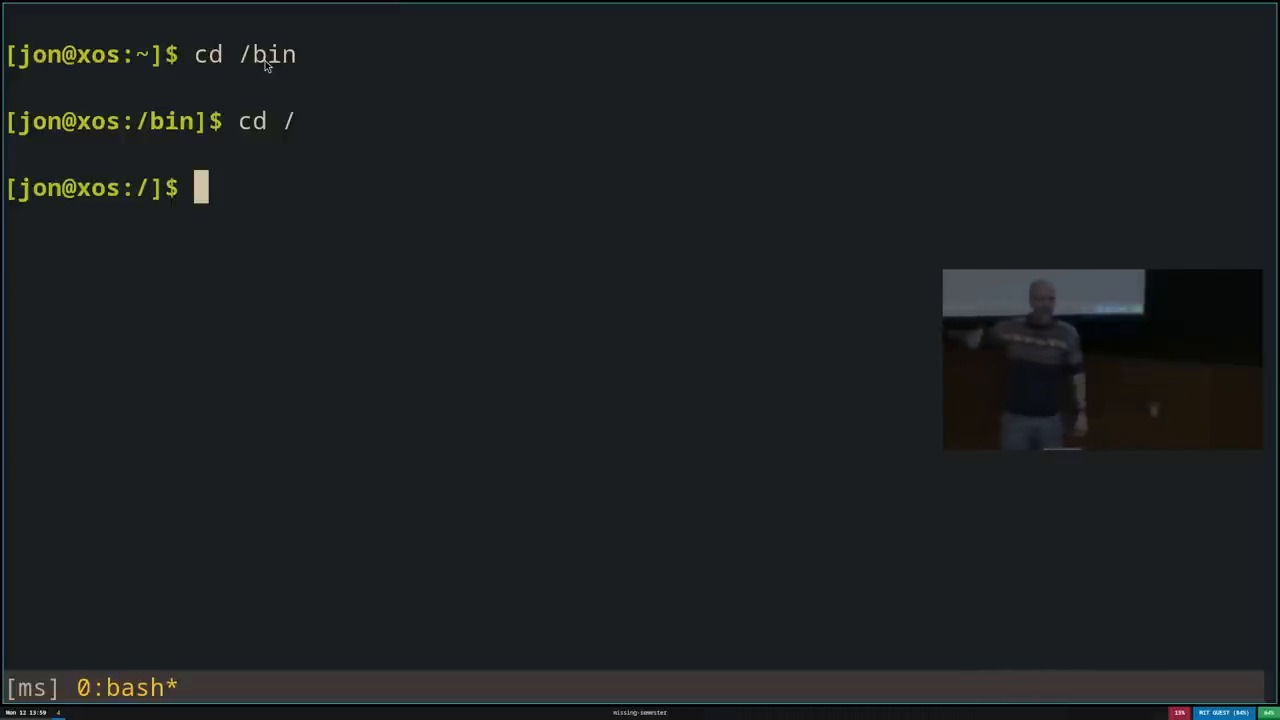
\includegraphics[width=0.92\textwidth]{figures/fig_06_cd_abs.jpg}
\caption{用 \texttt{cd /bin} 进入根目录下的 \texttt{bin}，提示符随之改变\vtag}
\end{figure}
\srcnote{00:23:00--00:23:15}
\end{minipage}


Shell 总有一个当前工作目录，提示符里已经显示了它。可以用 \texttt{cd}（change directory）切换到另一个目录，后面跟一个路径。以斜杠开头的路径是绝对路径。讲者想进入文件系统根目录下的 \texttt{bin} 目录，执行 \texttt{cd /bin}，提示符变成了 \texttt{/bin} 而不是原来的主目录；也可以直接 \texttt{cd /} 进入根目录。很多命令默认在当前工作目录上操作。

\subsection{相对路径与特殊路径}

\noindent\begin{minipage}{\textwidth}
\begin{figure}[H]
\centering
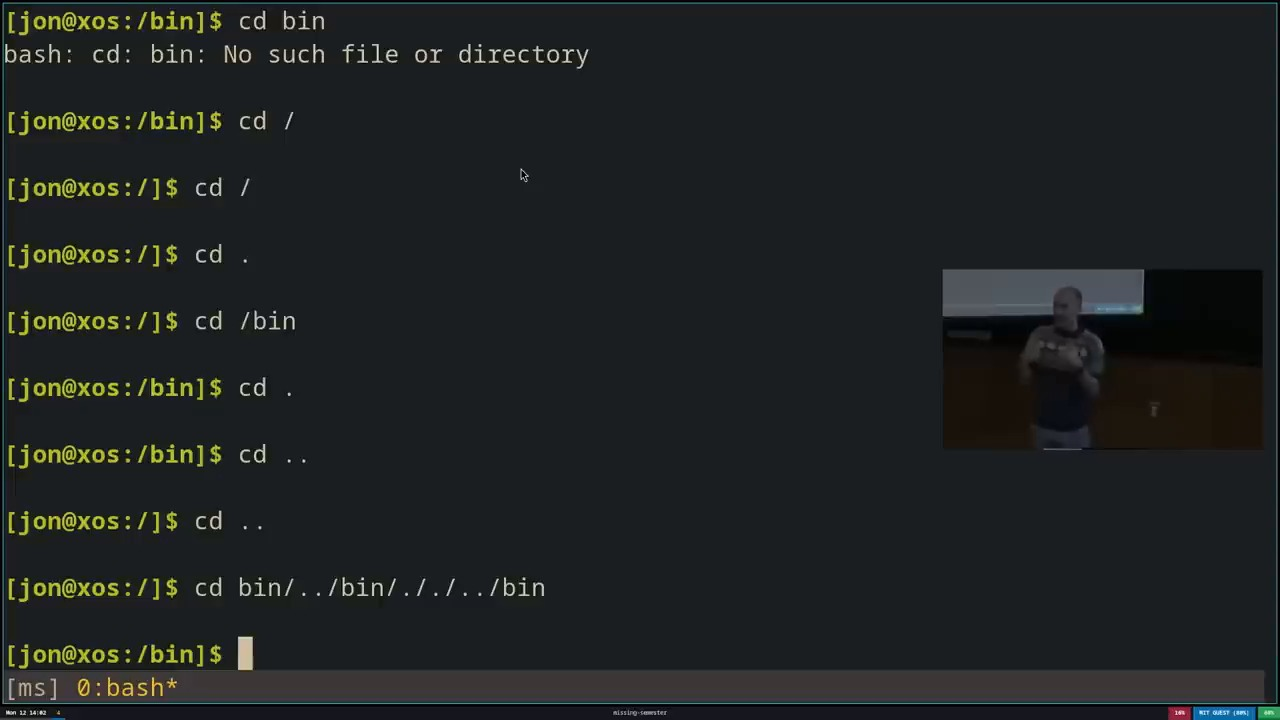
\includegraphics[width=0.92\textwidth]{figures/fig_07_cd_rel.jpg}
\caption{\texttt{.} 和 \texttt{..} 可以组合成任意复杂的相对路径\vtag}
\end{figure}
\srcnote{00:25:30--00:25:45}
\end{minipage}


讲者说，如果每次都要输入像 \texttt{/home/jon/dev/project/6824/version1/} 这样很长的路径，会非常麻烦。所以可以先 \texttt{cd} 进想工作的目录，再使用相对路径。相对路径是不以斜杠开头的路径，解析方式是：在当前工作目录中查找第一个路径分量（即以斜杠分隔的各部分），再从那里沿着斜杠继续往下，而不是从文件系统的根开始。例如在根目录下输入 \texttt{cd bin} 就进入 \texttt{/bin}；而在 \texttt{/bin} 里再 \texttt{cd bin} 会报告没有这个目录。

还有两个特殊的路径分量：点和点点。点 \texttt{.} 表示当前目录，\texttt{cd .} 会回到原地；点点 \texttt{..} 表示上一级目录。它们可以组合，例如 \texttt{cd bin/../bin/./.} 最后仍落在 \texttt{/bin}。讲者举例说明用处：假设你在做 6.824 的项目，想从一个版本目录切到相邻的另一个版本，就可以写 \texttt{cd ../version2}。

\subsection{主目录与快速导航}

有同学问波浪线：\texttt{cd \textasciitilde} 会回到主目录。斜杠是路径分量的分隔符，分隔解析路径时的每一步：\texttt{cd a/b/c} 的意思是进入 \texttt{a}，再进入 \texttt{b}，再进入 \texttt{c}，也就是进入 \texttt{a} 里的 \texttt{b} 里的 \texttt{c}。这些路径也可以和波浪线组合。

讲者提到还有更高效的导航方式：讲义里提到 zoxide，它记住你 \texttt{cd} 过的所有路径，让你更快地跳到其中任意一个，而不必在整个文件系统中一级级移动。还有一个技巧是 Tab 补全：输入路径或命令的一部分后按 Tab，Shell 会帮你补全。

\begin{practicebox}{路径练习}
讲义作者整理：设当前目录是 \texttt{/home/jon/dev}，判断以下命令之后所在的目录：\texttt{cd ..}；\texttt{cd ./project}；\texttt{cd \textasciitilde/dev/../dev}；\texttt{cd /}。再用 \texttt{pwd} 验证你的答案，\texttt{pwd} 会打印当前工作目录。
\end{practicebox}

\subsection{本章小结}

绝对路径从根目录出发，相对路径从当前目录出发，\texttt{.}、\texttt{..}、\textasciitilde{} 是三个特殊位置。下一个问题是：输入 \texttt{date} 时，Shell 怎么知道要运行哪个程序？

\section{Shell 怎样找到程序}

\subsection{PATH 环境变量}

\noindent\begin{minipage}{\textwidth}
\begin{figure}[H]
\centering
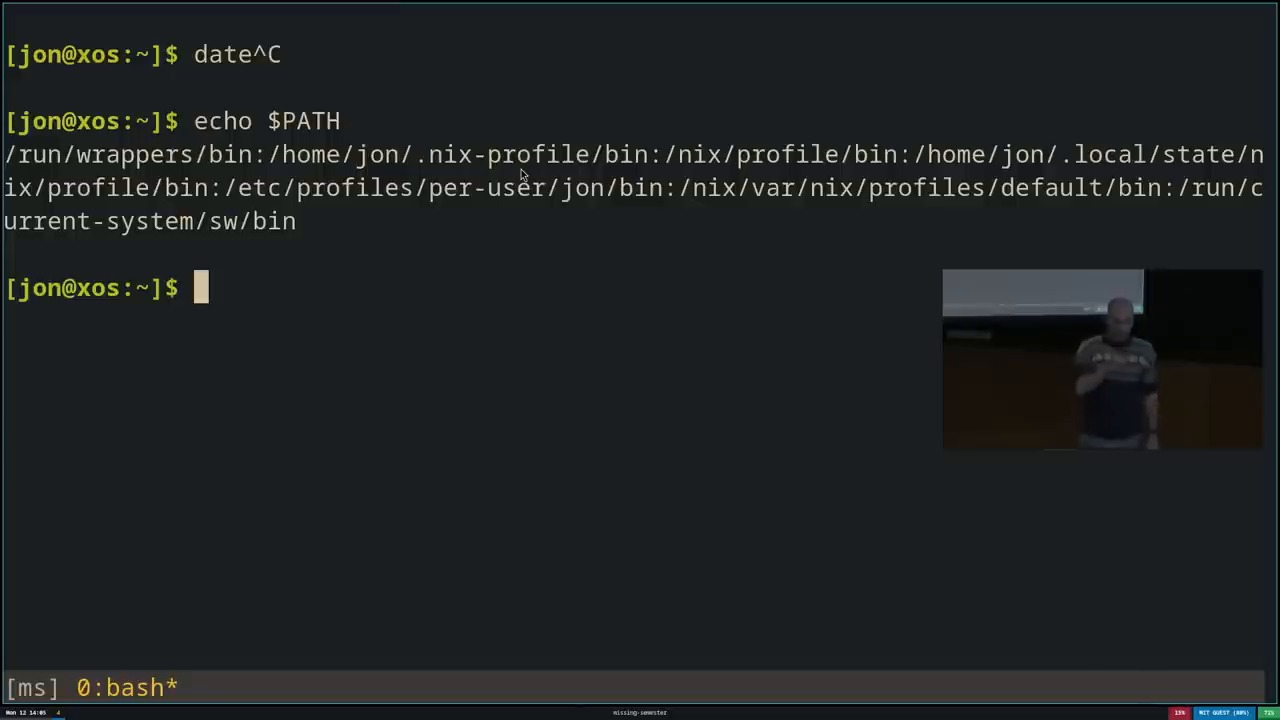
\includegraphics[width=0.92\textwidth]{figures/fig_08_path_var.jpg}
\caption{\texttt{echo \$PATH} 显示以冒号分隔的一串目录\vtag}
\end{figure}
\srcnote{00:29:00--00:29:15}
\end{minipage}


到目前为止我们用过 \texttt{echo}、\texttt{date}、\texttt{man} 和 \texttt{cd}。可是还有哪些程序可用？输入 \texttt{date} 时，Shell 又怎么知道要运行哪个程序，\texttt{date} 在电脑上的什么地方？讲者解释：在 Shell 里输入一个程序名时，Shell 会拿着这个名字去一个叫 \texttt{PATH} 的东西里查找。\texttt{PATH} 是一个环境变量，用 \texttt{echo \$PATH} 可以看到它的值：一串以冒号分隔的目录。运行程序时，Shell 逐个检查这些目录，寻找与程序同名的文件，找到就运行，否则看下一个。

\subsection{which}

\noindent\begin{minipage}{\textwidth}
\begin{figure}[H]
\centering
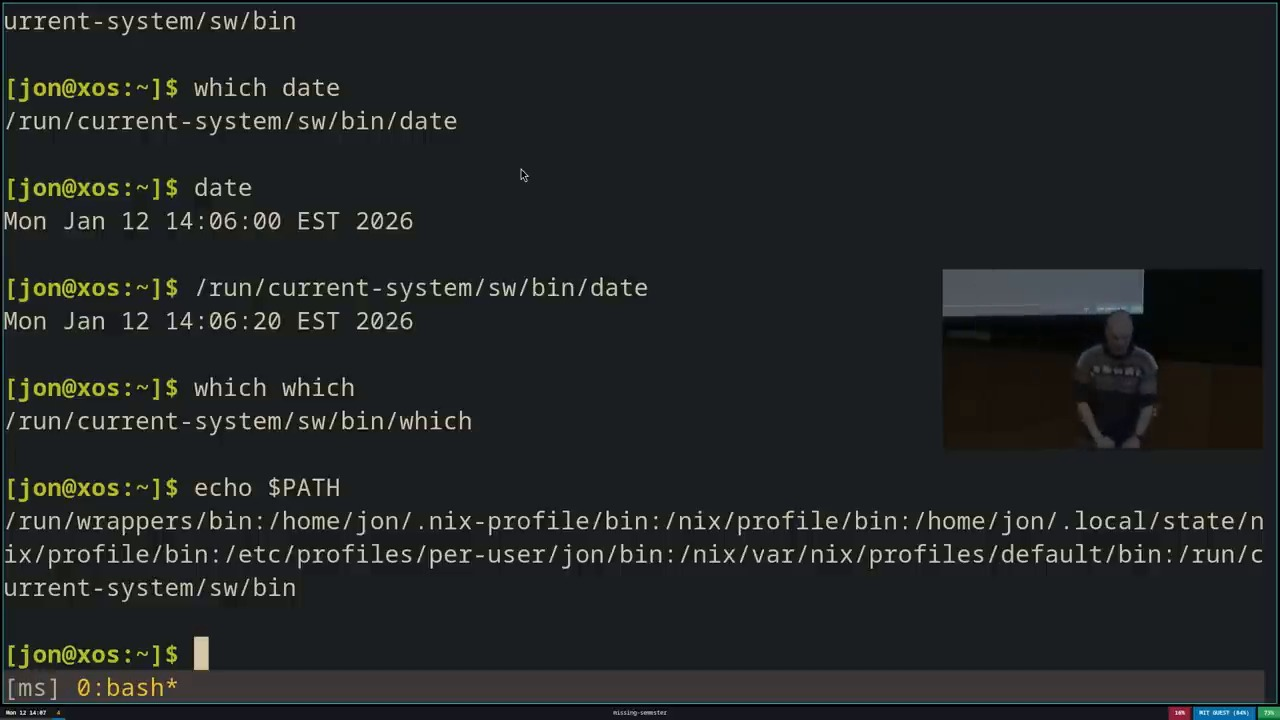
\includegraphics[width=0.92\textwidth]{figures/fig_09_which.jpg}
\caption{\texttt{which date} 和 \texttt{which which} 给出程序所在的具体路径\vtag}
\end{figure}
\srcnote{00:31:00--00:31:15}
\end{minipage}


我们可以对此进行检查。\texttt{which} 是一个程序，它沿着 \texttt{PATH} 列表查找，打印出第一次找到给定程序的位置。\texttt{which date} 显示了 \texttt{date} 命令所在的路径，所以运行 \texttt{date} 时实际执行的就是那个文件，直接输入完整路径也能运行它。\texttt{which} 本身也只是一个程序，\texttt{which which} 告诉我们它和 \texttt{date} 在同一个目录。讲者提醒，这个路径在你的机器上可能不同，取决于你的操作系统把软件装在哪里。

有同学问输入不完整的路径时，Shell 是不是在当前目录的上级目录里找。讲者说不是，它只在 \texttt{PATH} 列出的目录里找。如果同名程序在 \texttt{PATH} 中出现多次，Shell 执行按顺序遇到的第一个。可以用 \texttt{which -a} 列出所有副本：\texttt{echo} 和 \texttt{rustc} 都只有一个，而 \texttt{sh} 在他的 \texttt{PATH} 中出现在两个地方。

\noindent\begin{minipage}{\textwidth}
\begin{figure}[H]
\centering
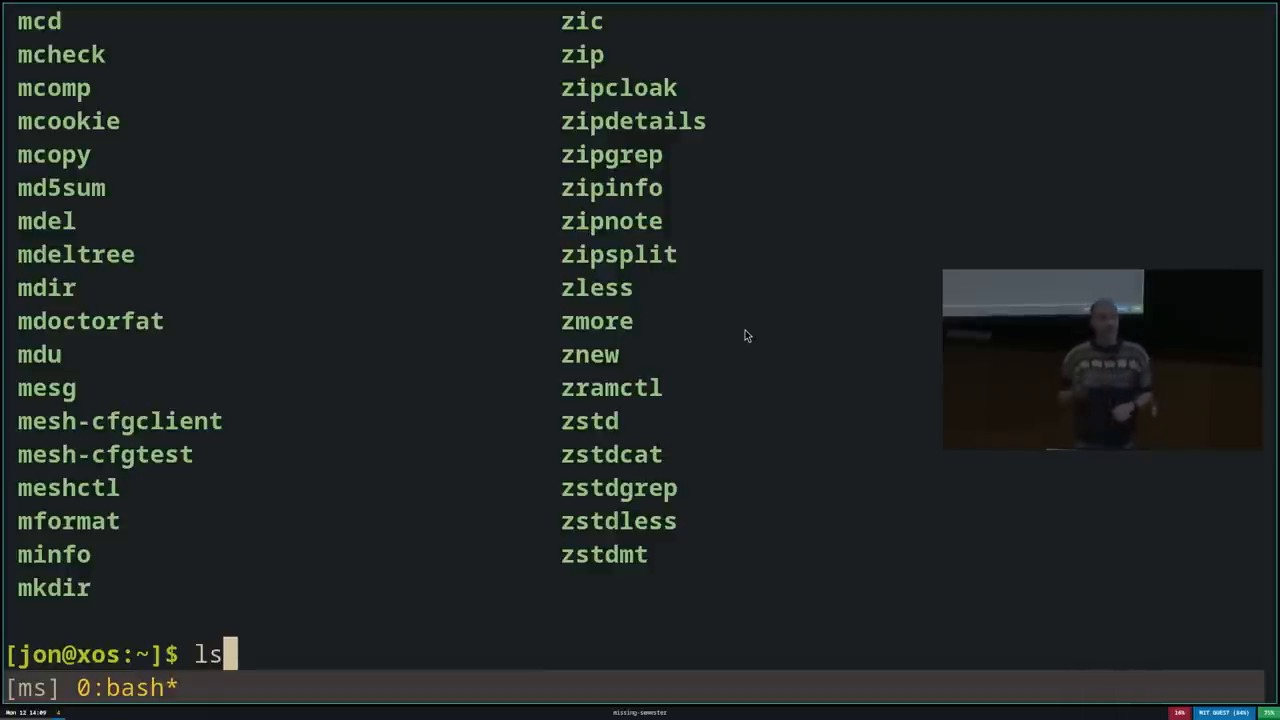
\includegraphics[width=0.92\textwidth]{figures/fig_10_ls_path.jpg}
\caption{列出 \texttt{PATH} 中某个目录的内容，就看到了一大批可用的程序\vtag}
\end{figure}
\srcnote{00:32:45--00:33:00}
\end{minipage}


这也给出了一个办法来了解自己有哪些程序：遍历 \texttt{PATH} 里的所有目录，列出每个目录的内容，就是全部程序。你也许不知道它们都是做什么的，但可以查手册页去探索。讲者用 \texttt{ls} 列出了其中一个目录。\texttt{ls} 是另一个程序，列出目录的内容，默认列出当前工作目录。

\begin{warningbox}{当前目录不在 PATH 中}
讲者在课的最后提到，如果把当前目录放进 \texttt{PATH}，那么当前目录里一个叫 \texttt{ls} 的文件就会取代系统的 \texttt{ls}。讲义作者补充：这正是默认不把当前目录放进 \texttt{PATH} 的原因之一，所以运行当前目录下的脚本要写 \texttt{./script.sh}。
\end{warningbox}

\subsection{本章小结}

Shell 按 \texttt{PATH} 中的目录顺序查找程序，\texttt{which} 能告诉你最终运行的是哪一个文件。知道了程序从哪里来，接下来认识一批最常用的程序。

\section{常用命令行程序}

\subsection{cat、sort、uniq、head、tail}

\noindent\begin{minipage}{\textwidth}
\begin{figure}[H]
\centering
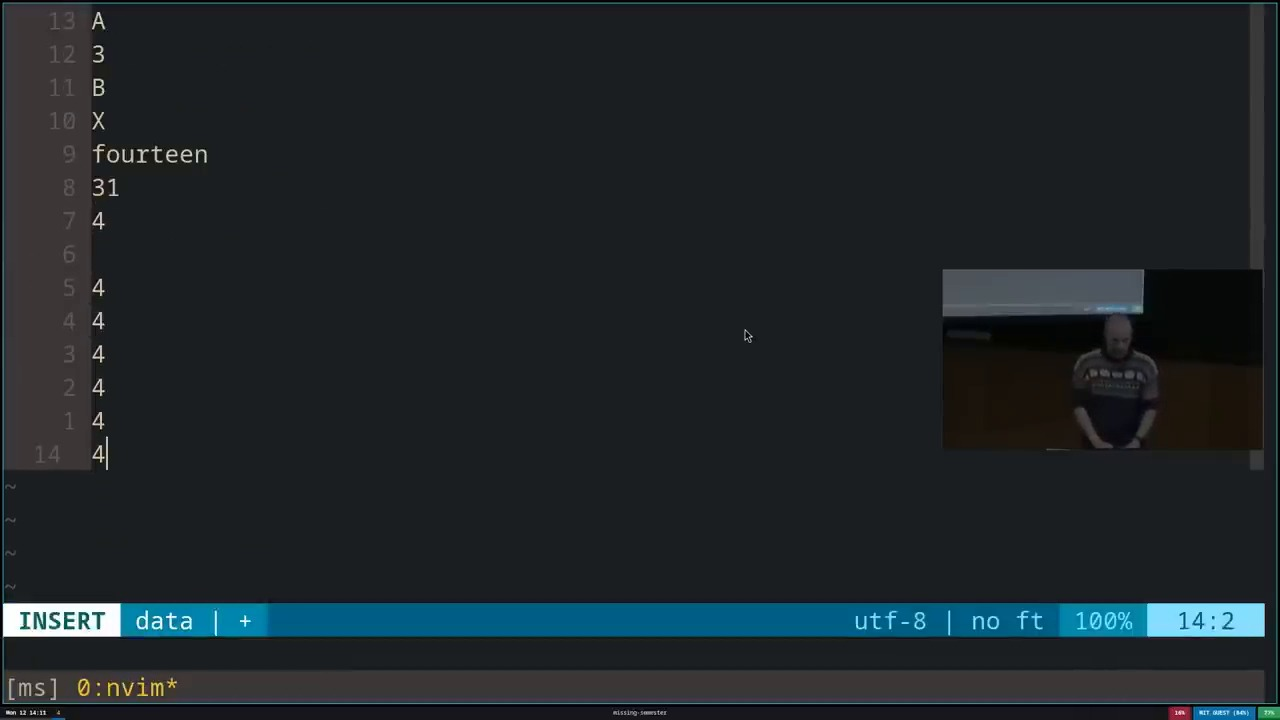
\includegraphics[width=0.92\textwidth]{figures/fig_11_sort.jpg}
\caption{\texttt{sort} 默认按字典序排序，所以 31 排在 4 前面\vtag}
\end{figure}
\srcnote{00:34:30--00:34:45}
\end{minipage}


\texttt{cat} 打印文件的内容，直接把它倒到终端里。\texttt{sort} 读取输入或参数指定的文件，按排序后的顺序打印各行。讲者在一个数据文件里加了 31 来说明一点：\texttt{sort} 默认按字典序排序，所以 3 后面跟着 31，这是按字母顺序的结果，按数值却未必正确；再加一个 4，会得到 3、31、4。可以给 \texttt{sort} 传参数改变这种行为。

\texttt{uniq} 去除重复行，但它并不聪明：它不会记住见过的每一行，只消除相邻的重复。可以把 \texttt{sort} 和 \texttt{uniq} 组合起来得到想要的效果，\texttt{sort} 也有 \texttt{-u} 选项，排序的同时去重。

\noindent\begin{minipage}{\textwidth}
\begin{figure}[H]
\centering
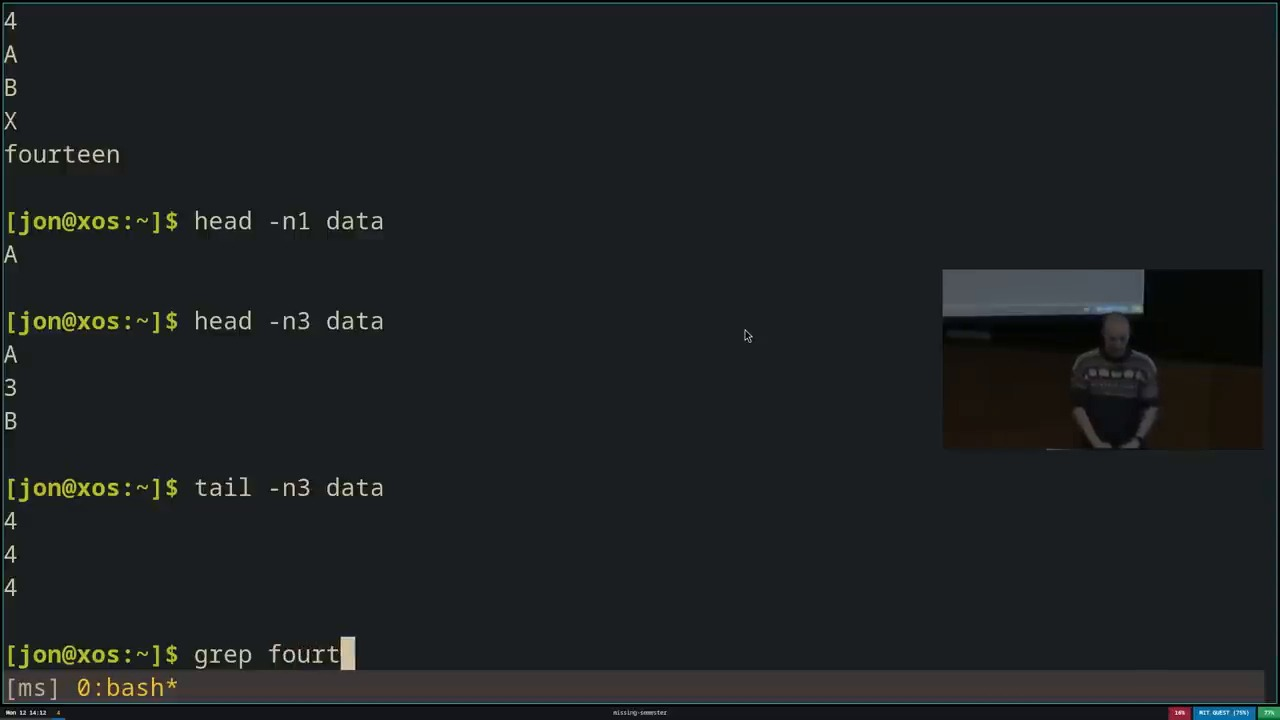
\includegraphics[width=0.92\textwidth]{figures/fig_12_head_tail.jpg}
\caption{\texttt{head -n} 和 \texttt{tail -n} 分别取文件开头和结尾的若干行\vtag}
\end{figure}
\srcnote{00:36:00--00:36:15}
\end{minipage}


\texttt{head} 打印文件的前 $n$ 行，默认 $n$ 是 $10$，可以用 \texttt{-n} 加一个数字指定；\texttt{tail} 打印最后 $n$ 行。

\begin{knowledgebox}{按数值排序}
讲义作者补充：\texttt{sort -n} 按数值排序，\texttt{sort -r} 逆序，\texttt{sort -k2,2} 只按第二列排序；与 \texttt{uniq -c}（统计每行出现次数）组合，就是统计频次的经典写法 \texttt{sort | uniq -c | sort -n}，后面的 SSH 日志例子正是这样做的。
\end{knowledgebox}

\subsection{grep}

\noindent\begin{minipage}{\textwidth}
\begin{figure}[H]
\centering
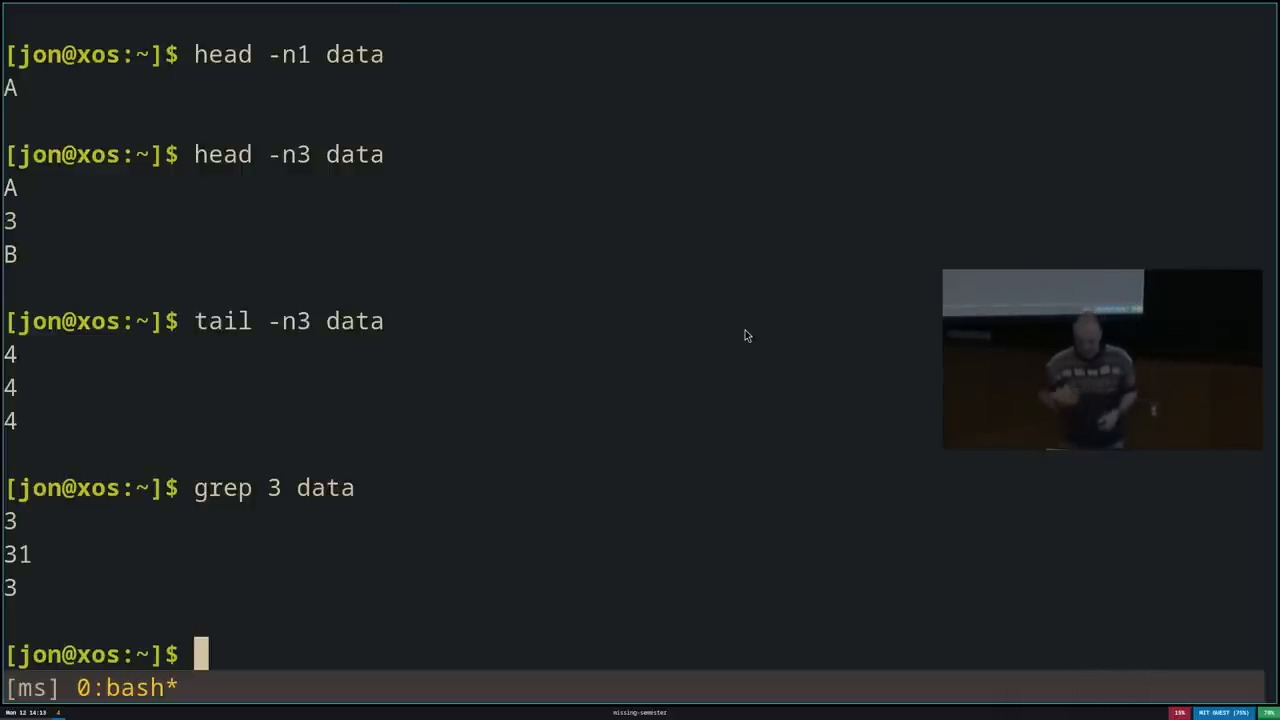
\includegraphics[width=0.92\textwidth]{figures/fig_13_grep.jpg}
\caption{\texttt{grep 3 data} 只打印包含 3 的行\vtag}
\end{figure}
\srcnote{00:37:00--00:37:15}
\end{minipage}


\texttt{grep} 在文件里查找匹配某个模式的内容。它接受两个参数：一个模式，以及要搜索的一个或一组文件，然后打印所有匹配的行。例如 \texttt{grep 3 data}，这些行包含 3，其余的不包含，就不打印。讲者说 \texttt{grep} 比看上去强大得多：模式可以是正则表达式，所以能在可能很大的目录里搜索相当复杂的东西。

\noindent\begin{minipage}{\textwidth}
\begin{figure}[H]
\centering
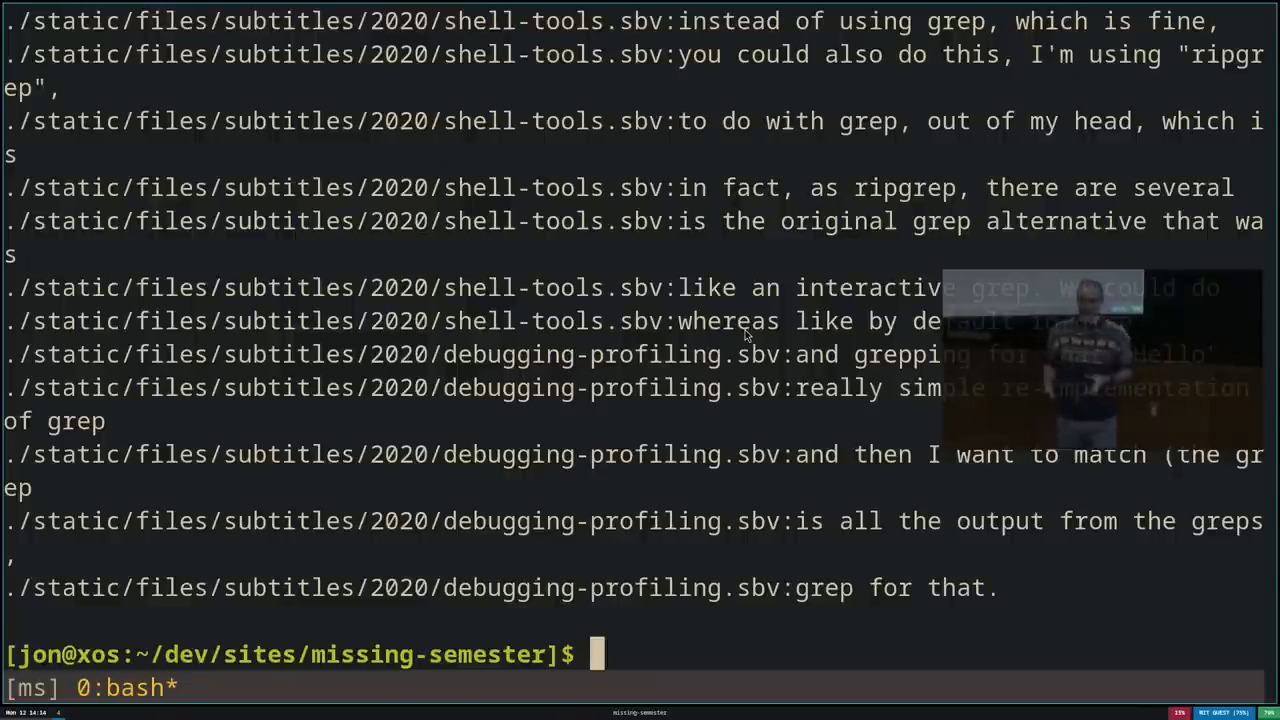
\includegraphics[width=0.92\textwidth]{figures/fig_14_grep_r.jpg}
\caption{在课程仓库里用 \texttt{grep -r} 递归搜索所有文件\vtag}
\end{figure}
\srcnote{00:38:00--00:38:15}
\end{minipage}


\texttt{grep} 除了搜索文件也能搜索目录。讲者进入课程网站的仓库，用 \texttt{grep -r grep .} 查找所有包含“grep”的地方，\texttt{-r} 表示递归，深入所有嵌套的文件夹，从当前目录开始搜索所有文件。

\subsection{sed 与正则表达式}

\noindent\begin{minipage}{\textwidth}
\begin{figure}[H]
\centering
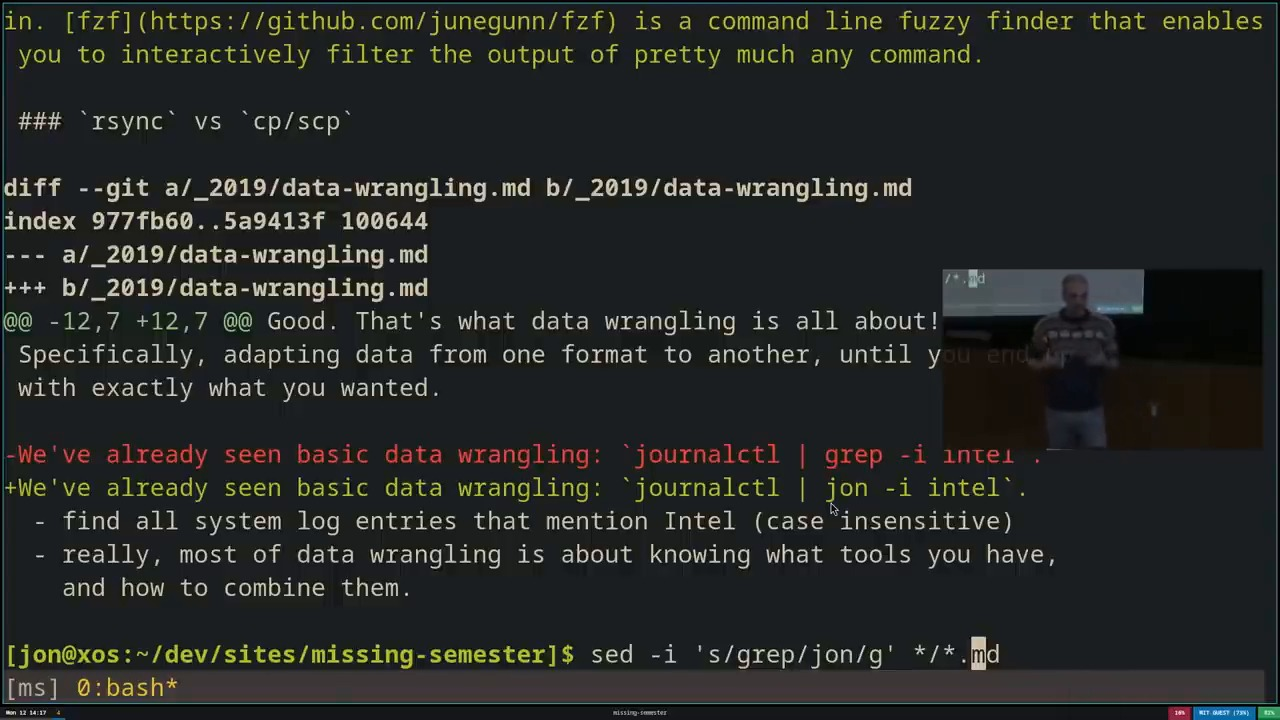
\includegraphics[width=0.92\textwidth]{figures/fig_15_sed.jpg}
\caption{\texttt{sed -i 's/grep/john/g'} 对所有 Markdown 文件做全局替换\vtag}
\end{figure}
\srcnote{00:40:30--00:40:45}
\end{minipage}


\texttt{sed} 的有趣之处在于它有自己的编程语言，可以编程控制它怎样编辑文件。但通常它用于很简单的任务，例如查找替换。讲者想把每个 grep 都替换成 john，就用 \texttt{sed -i}，\texttt{-i} 表示就地替换，不创建新文件，而是直接修改原文件。替换命令 \texttt{s/grep/john/} 中，\texttt{s} 表示替换，两个斜杠分隔匹配模式和替换内容；末尾加 \texttt{g} 表示全局替换，否则一行里出现两次 grep 时只会替换第一个。文件参数 \texttt{**/*.md} 是一个通配符，意思是在任何目录中寻找以 \texttt{.md} 结尾的文件，课程网站的文件都是这种格式。运行后执行 \texttt{git diff}，可以看到一大片改动。

\begin{lstlisting}[language=bash]
sed -i 's/grep/john/g' **/*.md
\end{lstlisting}

有同学问通配符和传给 \texttt{grep} 的正则表达式有什么关系。讲者解释：正则表达式和通配符都是表达模式的方式，但通常是由特定程序而不是 Shell 本身支持的。在 \texttt{grep} 和 \texttt{sed} 命令里，正则表达式就是 \texttt{grep} 或 \texttt{sed} 支持的东西；而用来指定路径的通配符则由 Shell 处理。Shell 一般不支持对路径使用正则表达式，路径上通常只能用通配符。讲者说正则表达式用在路径上本来就别扭，因为路径关心目录和文件，而正则表达式没有这个概念，只是拿一段文本去匹配模式；在通配符里，斜杠则确实表示目录分隔。他还在 \texttt{sed} 里写了一个更复杂的正则表达式，例如“任意一个不是 a 的字符，跟着任意多个字符，然后一个短横线，再跟一个数字”，并说现在不指望大家学会正则表达式。

\begin{importantbox}{通配符与正则表达式的分工}
通配符是一种很简单的模式语言，由 Shell 用来匹配文件路径，例如 \texttt{*.py}、\texttt{**/*.md}；正则表达式是复杂得多的模式语言，由 \texttt{grep}、\texttt{sed}、\texttt{awk} 等程序用来匹配文本内容。同样一个星号，在通配符里表示“任意字符串”，在正则表达式里表示“前一个字符重复任意次”。
\end{importantbox}

\subsection{find}

\noindent\begin{minipage}{\textwidth}
\begin{figure}[H]
\centering
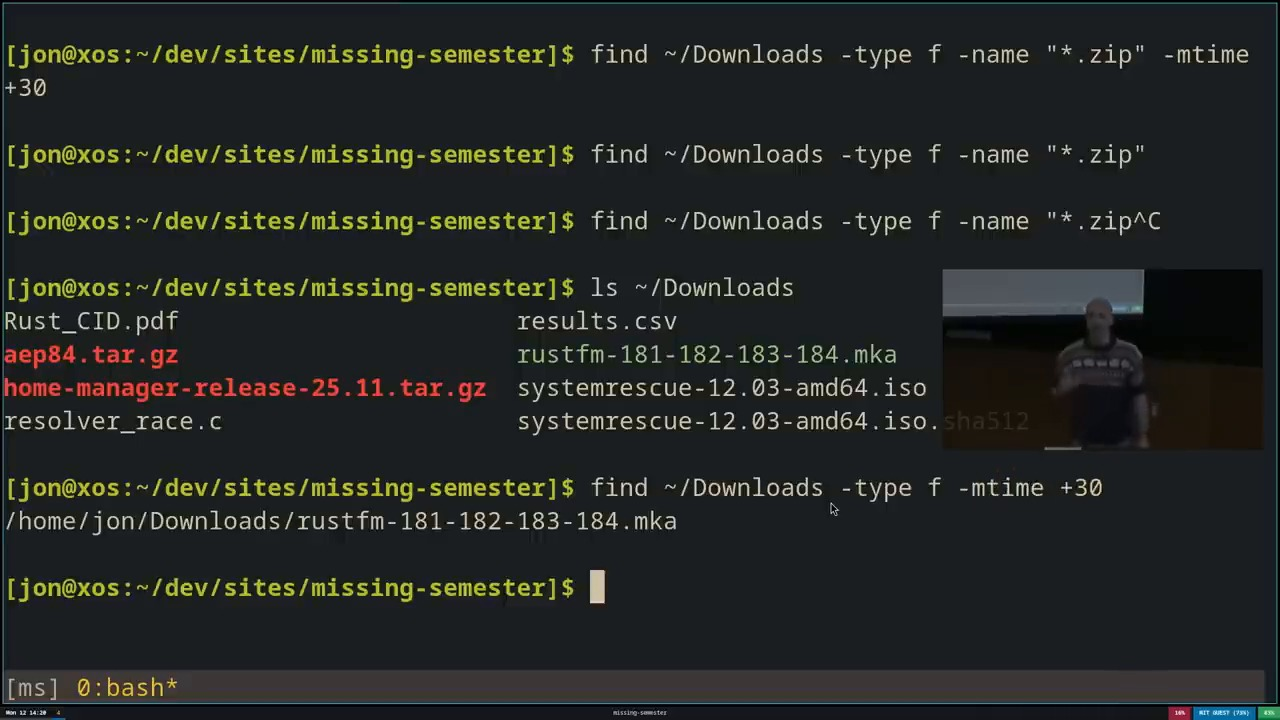
\includegraphics[width=0.92\textwidth]{figures/fig_16_find.jpg}
\caption{\texttt{find \textasciitilde/Downloads -type f -name "*.zip" -mtime +30} 找出超过 30 天的压缩包\vtag}
\end{figure}
\srcnote{00:44:00--00:44:15}
\end{minipage}


下一个程序是 \texttt{find}，它查找文件：告诉它你要找什么样的文件，它就在你指定的位置搜索符合条件的文件。例如在下载目录里查找类型为普通文件（\texttt{-type f}，与目录相对）、名字以 \texttt{.zip} 结尾的东西。再加上 \texttt{-mtime +30}，就只要超过 30 天的文件，他的下载目录里只有一个文件满足。\texttt{find} 有一整套参数语言，可以用 \texttt{man find} 学习：可以按大小、按新旧程度等各种条件搜索。

\noindent\begin{minipage}{\textwidth}
\begin{figure}[H]
\centering
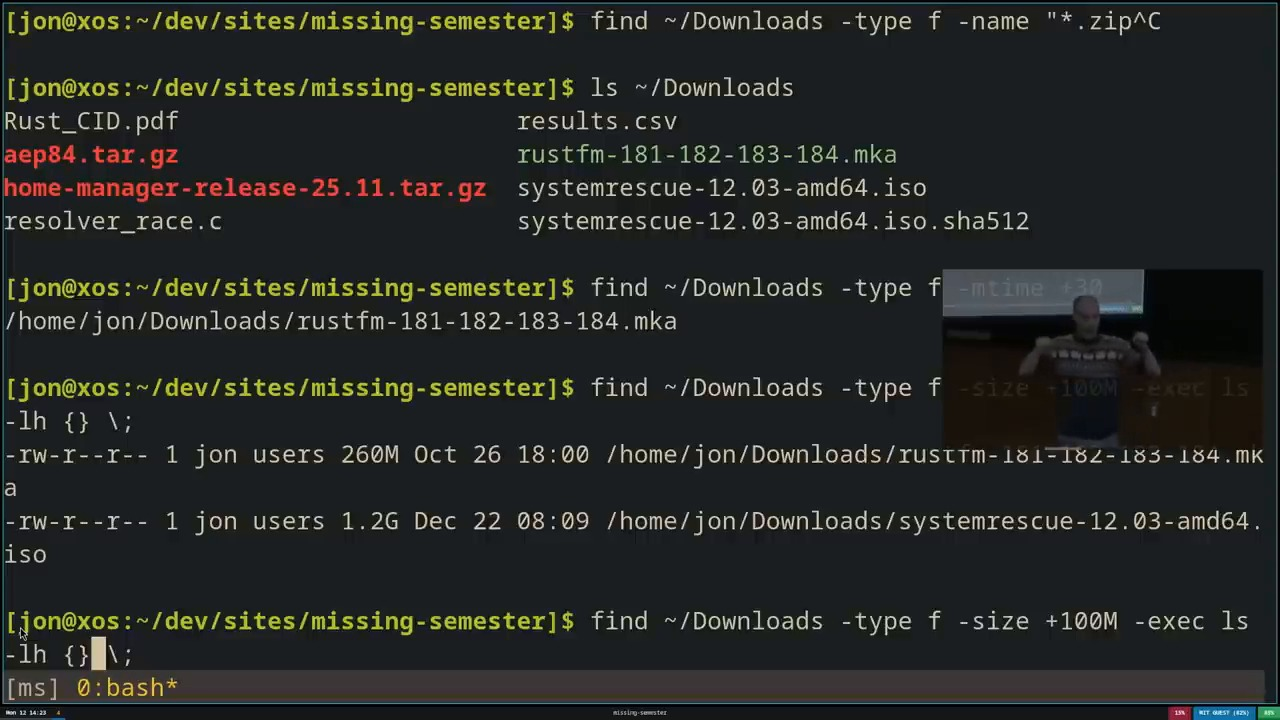
\includegraphics[width=0.92\textwidth]{figures/fig_17_find_exec.jpg}
\caption{\texttt{find} 的 \texttt{-exec} 对每个匹配的文件执行 \texttt{ls -lh}\vtag}
\end{figure}
\srcnote{00:46:30--00:46:45}
\end{minipage}


\texttt{find} 还能对找到的每个文件执行命令。讲者写了 \texttt{find \textasciitilde -type f -size +100M -exec ls -lh \{\} \textbackslash;}，意思是：对每个大于 100M 的文件运行 \texttt{ls}，\texttt{-l} 显示更多信息，\texttt{-h} 用人类易读的格式显示大小，即用 G、M、K 而不是字节数。\texttt{\{\}} 会被替换为匹配文件的路径。末尾的反斜杠分号是因为：假如想在后面再给 \texttt{find} 自己加参数，比如 \texttt{-mtime +30}，\texttt{find} 怎么知道哪些参数属于 \texttt{-exec} 的命令、哪些属于自己？它不知道。所以用分号标记 \texttt{-exec} 参数列表的结束，而分号对 Shell 有特殊含义，需要像转义空格那样转义。讲者说这是 \texttt{find} 特有的写法，其他程序有别的方式。

他又展示了一条命令但故意没有执行：它会删除下载目录里所有至少 100M、并且放了至少 30 天的文件，一条命令全部完成。他解释，有时他输入一条命令却不执行，直接跳到下一行，用的就是 Ctrl+C，它表示取消当前的输入或命令。

\noindent\begin{minipage}{\textwidth}
\begin{figure}[H]
\centering
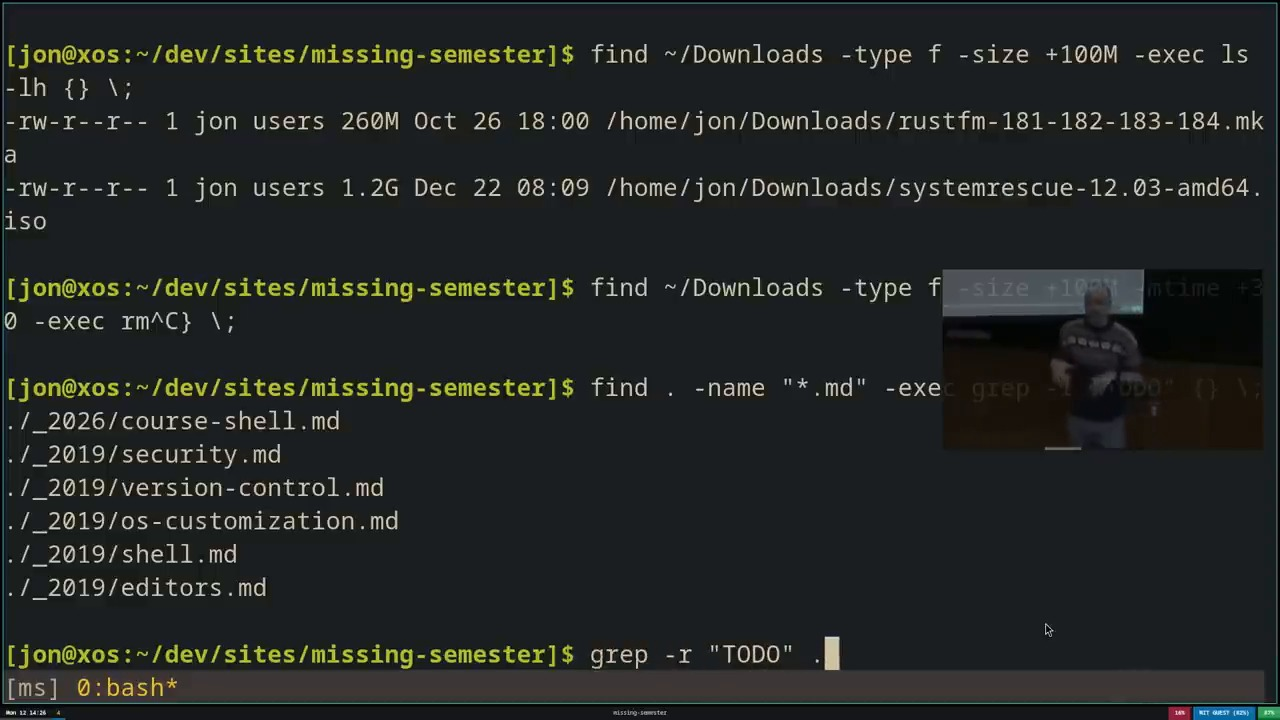
\includegraphics[width=0.92\textwidth]{figures/fig_18_find_todo.jpg}
\caption{\texttt{find} 配合 \texttt{grep -l} 列出所有写着 TODO 的 Markdown 文件\vtag}
\end{figure}
\srcnote{00:49:30--00:49:45}
\end{minipage}


另一个例子是 \texttt{find . -name "*.md" -exec grep -l TODO \{\} \textbackslash;}：对当前目录下的每个 Markdown 文件运行 \texttt{grep}，模式是 TODO，\texttt{-l} 表示打印匹配的文件名而不是匹配的行。这样就能知道哪些文件里写了 TODO，编程时想找“以后要回来做的事”很有用。

\noindent\begin{minipage}{\textwidth}
\begin{figure}[H]
\centering
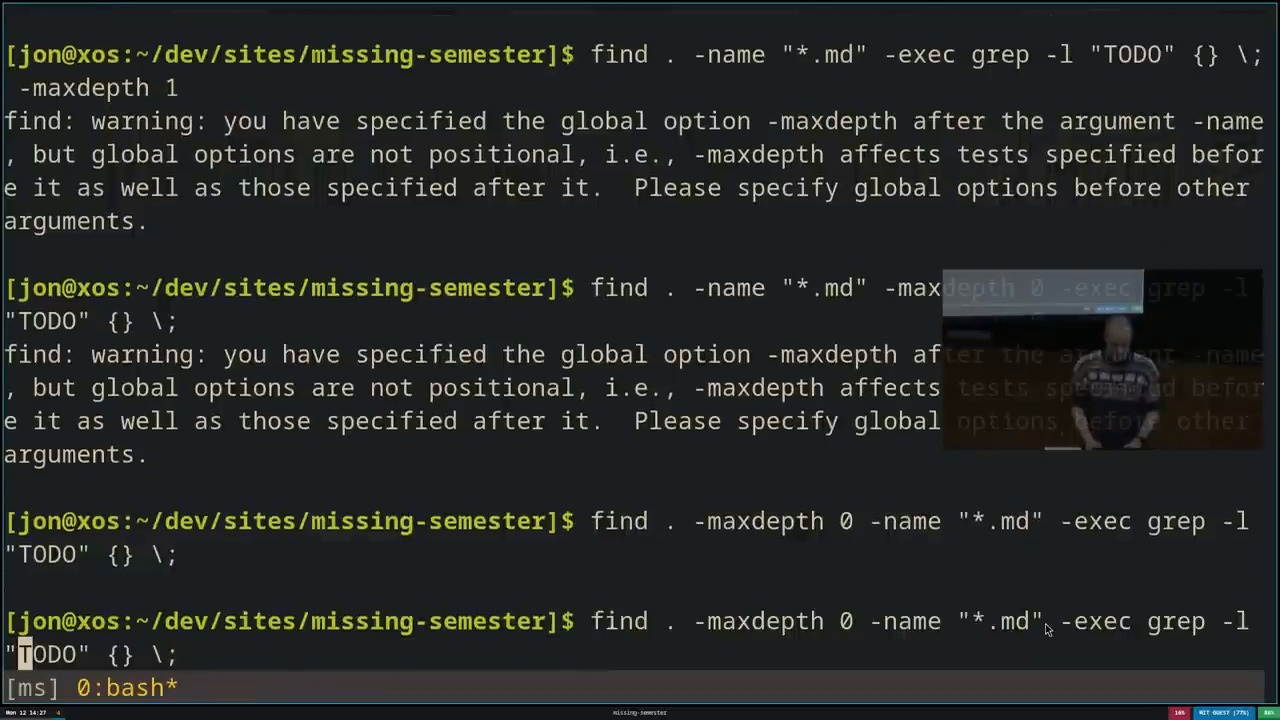
\includegraphics[width=0.92\textwidth]{figures/fig_19_maxdepth.jpg}
\caption{\texttt{-maxdepth} 必须放在其他条件之前，否则 \texttt{find} 会给出警告\vtag}
\end{figure}
\srcnote{00:51:00--00:51:15}
\end{minipage}


讲者说 \texttt{find} 的语法有点吓人，这也正是值得问 LLM 的地方：网上有大量 \texttt{find} 命令的例子，LLM 通常能轻松写出大致符合要求的命令。讲义里还链接了更现代、更顺手、更不易误用的工具，比如 \texttt{fd}。有同学问 \texttt{find} 是否默认递归：是的。讲者演示 \texttt{-maxdepth}：\texttt{-maxdepth 0} 和 \texttt{1} 都没有结果，取 \texttt{2} 才找到；而且把它放在 \texttt{-name} 之后时，\texttt{find} 会警告说这个全局选项应该放在其他参数前面。他的评价是：\texttt{find} 很烦人。

\begin{warningbox}{先预览，再执行破坏性操作}
讲义作者提醒：在 \texttt{find} 后面接 \texttt{-delete} 或 \texttt{-exec rm} 之前，先不带删除动作运行一遍，确认列出的确实是想删的文件；名字模式一定要加引号，例如 \texttt{-name "*.zip"}，否则 Shell 可能先把星号展开成当前目录的文件名。
\end{warningbox}

\subsection{awk}

\noindent\begin{minipage}{\textwidth}
\begin{figure}[H]
\centering
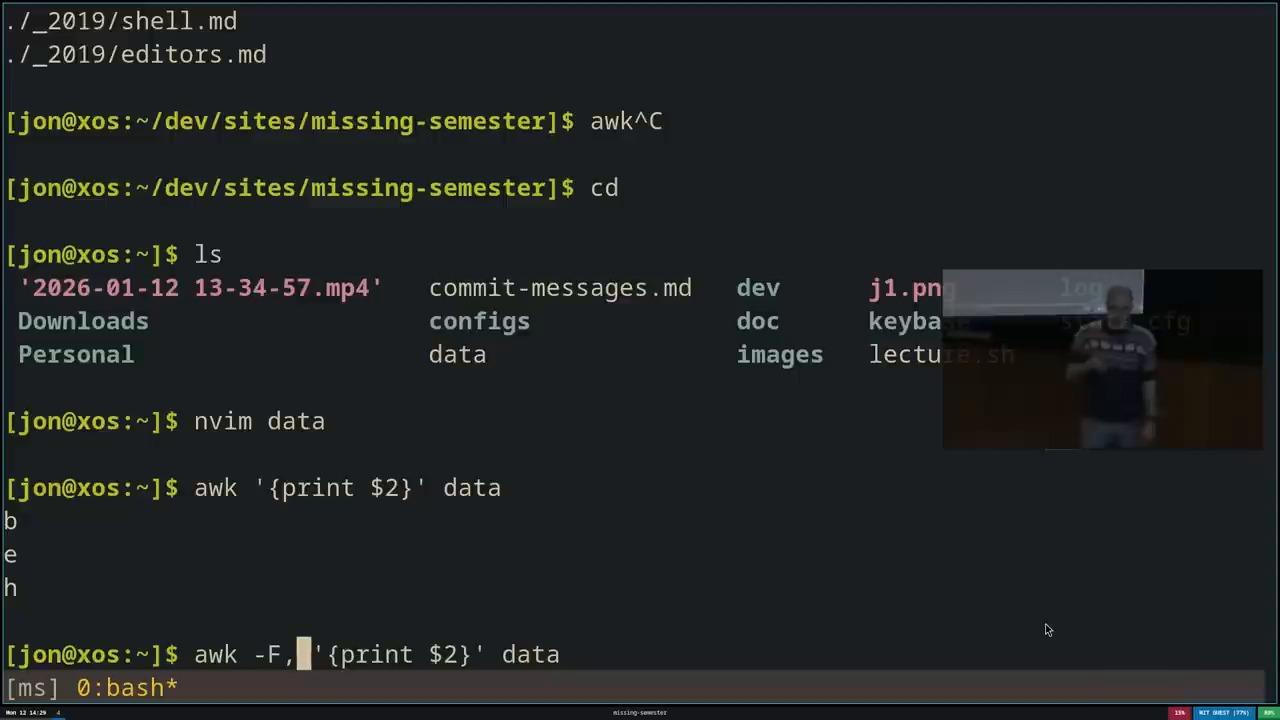
\includegraphics[width=0.92\textwidth]{figures/fig_20_awk.jpg}
\caption{\texttt{awk '\{print \$2\}'} 打印每行的第二列，\texttt{-F,} 把分隔符改成逗号\vtag}
\end{figure}
\srcnote{00:53:00--00:53:15}
\end{minipage}


接下来是 \texttt{awk}（A-W-K）。和 \texttt{sed} 一样，它内置了自己的编程语言，但 \texttt{sed} 用于编辑文件，\texttt{awk} 用于解析文件：默认按空白和换行切分文件，然后让你对各列进行操作。\texttt{awk '\{print \$2\}' data} 打印每一行的第二列。讲者说不会在这里教 \texttt{awk} 的整个语言，那相当庞大，但只要学几个关键点就能做很简单的事：花括号表示要执行的代码块，花括号前面还可以写一个模式，表示只对匹配的行执行。

如果用 \texttt{-F,} 把分隔符改成逗号，它就变成了一个 CSV 解析器：每行是一条记录，按逗号分成列。对他这个没有逗号的文件，这样就没有第二列了，因为所有内容都在第一列。有同学问 \texttt{awk} 是否用于张量处理：讲者说不是，虽然张量也可以看成行和列，但 \texttt{awk} 根本不理解二进制文件。

\subsection{组合起来：分析 SSH 日志}

\noindent\begin{minipage}{\textwidth}
\begin{figure}[H]
\centering
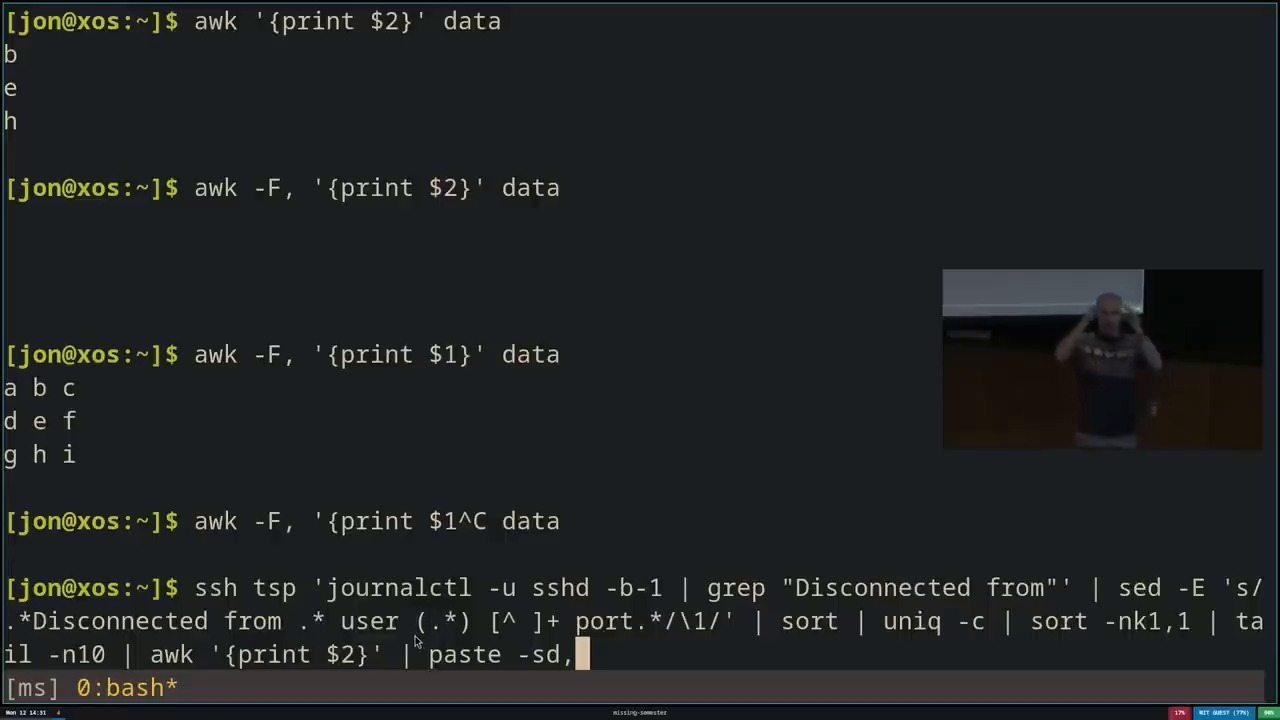
\includegraphics[width=0.92\textwidth]{figures/fig_21_ssh_pipeline.jpg}
\caption{一条组合了 \texttt{ssh}、\texttt{grep}、\texttt{sed}、\texttt{sort}、\texttt{uniq}、\texttt{awk} 与 \texttt{paste} 的长命令\vtag}
\end{figure}
\srcnote{00:54:30--00:54:45}
\end{minipage}


讲者展示了把这些程序组合起来的威力：

\begin{lstlisting}[language=bash]
ssh myserver 'journalctl -u sshd -b-1 | grep "Disconnected from"' \
  | sed -E 's/.*Disconnected from .* user (.*) [^ ]+ port.*/\1/' \
  | sort | uniq -c \
  | sort -nk1,1 | tail -n10 \
  | awk '{print $2}' | paste -sd,
\end{lstlisting}

它在远程服务器上运行 \texttt{journalctl}，打印 SSH 守护进程（也就是你远程连接时连上的那个东西）的日志，\texttt{-b -1} 表示只要上一次启动以来的日志，再用 \texttt{grep} 找出包含“Disconnected from”的行。然后交给 \texttt{sed}，用一个正则表达式把每一行替换成其中的用户名：任意字符、Disconnected from、空格、user、空格、任意字符（这就是用户名）、空格、一个非空格的串、空格、port，等等。讲者说这个表达式他写了好一阵，随着正则表达式越来越熟练，就会学会写这种模式。

接下来 \texttt{sort | uniq -c} 统计每个用户名出现的次数，\texttt{sort -nk1,1} 按包含计数的第一列做数值排序，最常见的排在最后；\texttt{tail -n10} 取最后 $10$ 个，也就是前 $10$ 名；\texttt{awk} 只打印用户名而不打印计数；最后 \texttt{paste -sd,} 把这些行粘成用逗号分隔的一行。讲者现场运行时服务器似乎宕机了，他说那是改天要修的事；请大家相信，它会打印出尝试登录他服务器最多的 $10$ 个用户名，其中没有一个是他的名字，全是垃圾连接。讲义里给出的结果是 \texttt{postgres,mysql,oracle,dell,ubuntu,inspur,test,admin,user,root}。\texttt{ssh} 是在远程机器上运行命令的方式，下一讲会详细讲。

\subsection{本章小结}

\texttt{cat}、\texttt{sort}、\texttt{uniq}、\texttt{head}、\texttt{tail}、\texttt{grep}、\texttt{sed}、\texttt{find}、\texttt{awk} 各自只做一件事，但组合起来能在一条命令里完成复杂的数据处理。把它们连在一起的，是接下来要讲的 Shell 语言本身。

\section{Shell 语言}

\subsection{管道与重定向}

\noindent\begin{minipage}{\textwidth}
\begin{figure}[H]
\centering
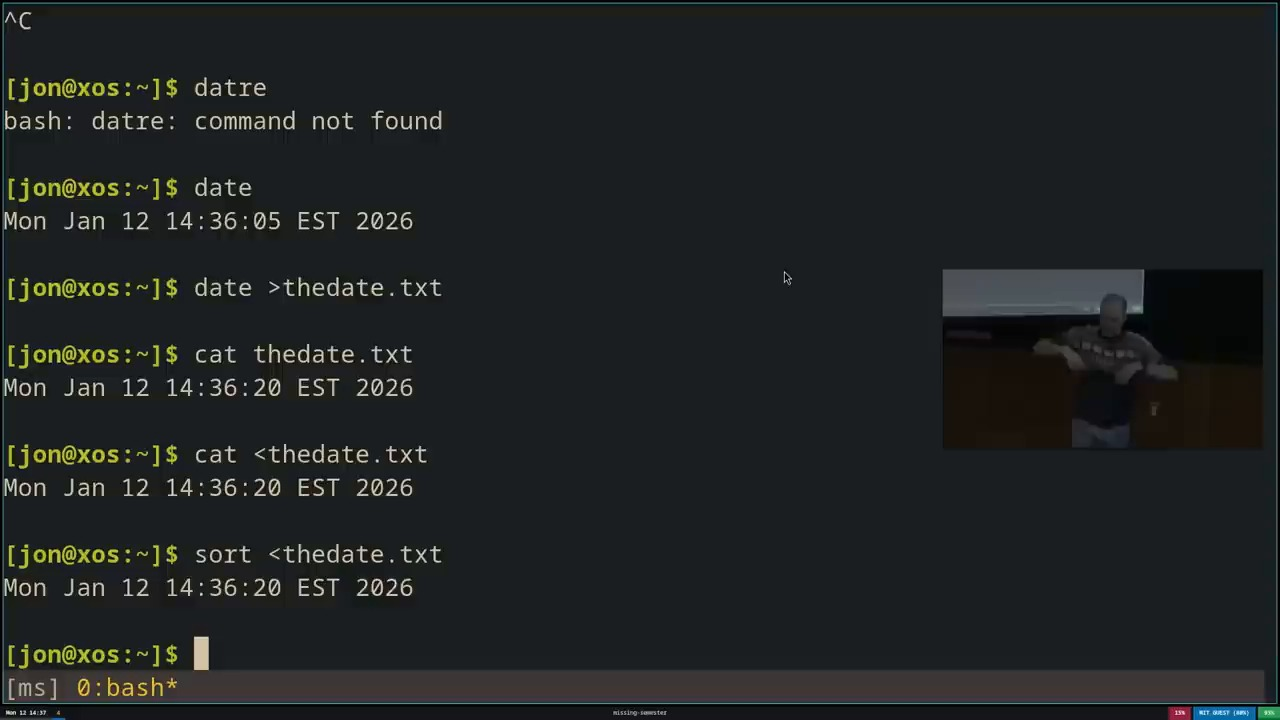
\includegraphics[width=0.92\textwidth]{figures/fig_22_redirect.jpg}
\caption{\texttt{>} 把 \texttt{date} 的输出写入文件，\texttt{<} 让 \texttt{cat} 从文件读取输入\vtag}
\end{figure}
\srcnote{01:00:30--01:00:45}
\end{minipage}


讲者指出，刚才的例子引入了一个新概念：竖线，即管道符。这是 bash 编程语言的一个构造，意思是运行左边的程序，把它的输出作为右边程序的输入。这是一种连接程序的方式，于是程序的输入不再是你的键盘，输出也不再是你的终端。

类似地，可以用尖括号重定向：\texttt{date > thedate.txt} 把 \texttt{date} 的输出写进文件而不是终端；反方向的尖括号表示不从终端而从某个位置读取输入，例如 \texttt{cat < thedate.txt}，对 \texttt{sort} 也一样，只是文件只有一行时排序没有效果。这让我们能重定向程序的输入和输出。

\begin{knowledgebox}{tee}
课程讲义还介绍了 \texttt{tee}：它把标准输入原样输出到标准输出，同时写入文件。例如 \texttt{verbose cmd | tee verbose.log | grep CRITICAL} 既把完整日志存进文件，又让终端只显示筛选后的关键信息。另外，\texttt{>>} 表示追加到文件而不是覆盖。
\end{knowledgebox}

\subsection{条件}

\noindent\begin{minipage}{\textwidth}
\begin{figure}[H]
\centering
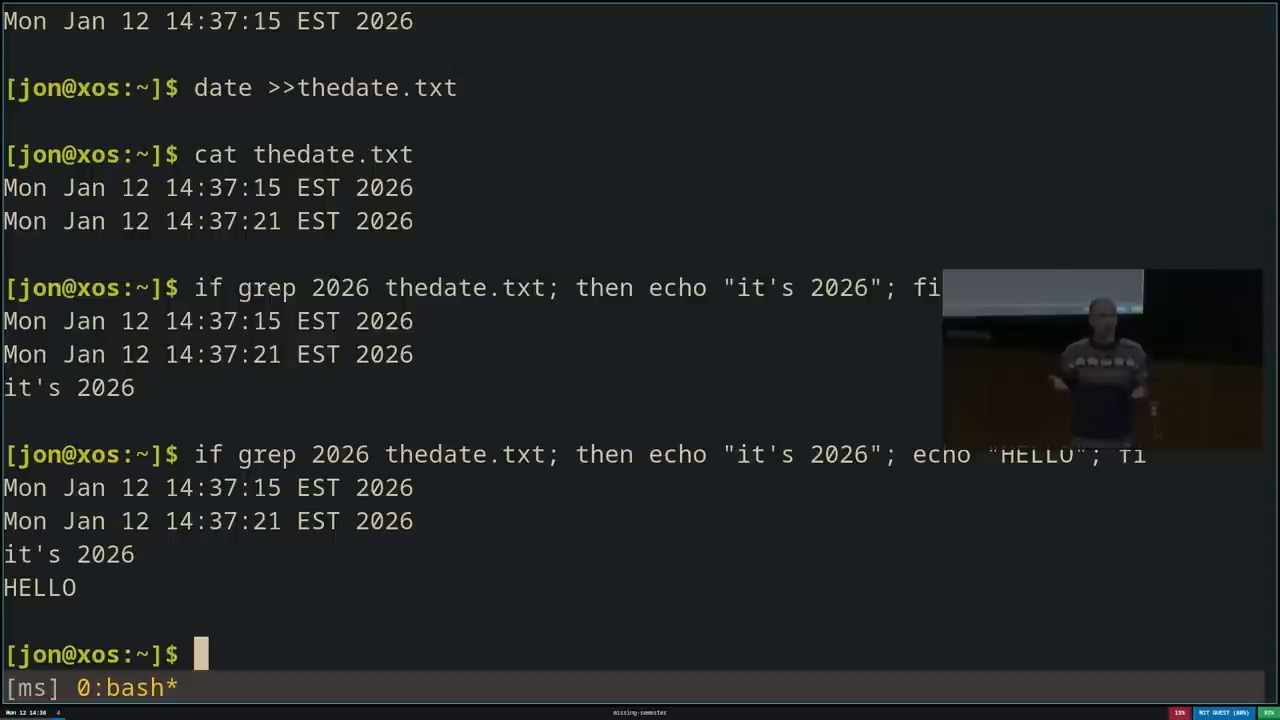
\includegraphics[width=0.92\textwidth]{figures/fig_23_if_grep.jpg}
\caption{\texttt{if grep 2026 thedate.txt; then echo ...; fi} 根据 \texttt{grep} 是否成功决定执行什么\vtag}
\end{figure}
\srcnote{01:02:00--01:02:15}
\end{minipage}


讲者说这里有一整门编程语言，没有时间全部讲完，只做一个非常快速的回顾。bash 有条件语句：\texttt{if grep 2026 thedate.txt; then echo "it's 2026"; fi}，它运行 \texttt{grep}，当且仅当 \texttt{grep} 成功退出时，才运行 \texttt{then} 后面的命令，也可以加 \texttt{else} 分支。结束 \texttt{if} 的方式是 \texttt{fi}，讲者笑说“为什么不呢”。怎么知道 \texttt{grep} 找到东西时成功退出？这也写在 \texttt{grep} 的手册里：在大多数 \texttt{grep} 手册中搜索 exit status，就能找到这个程序退出值的说明，\texttt{grep} 选中至少一行时退出码为 $0$。

\subsection{循环}

\noindent\begin{minipage}{\textwidth}
\begin{figure}[H]
\centering
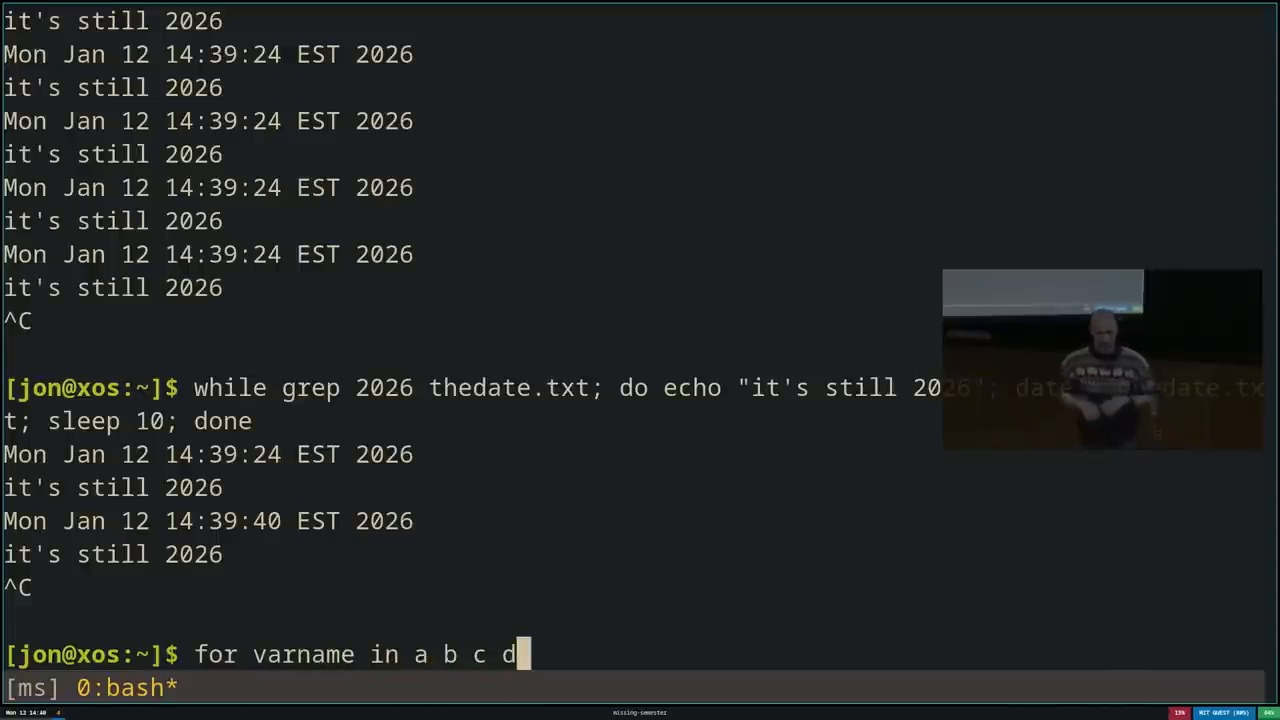
\includegraphics[width=0.92\textwidth]{figures/fig_24_while.jpg}
\caption{\texttt{while} 循环配合 \texttt{sleep 10} 每隔一段时间检查一次条件\vtag}
\end{figure}
\srcnote{01:03:30--01:03:45}
\end{minipage}


\texttt{while} 循环在命令保持为真的期间不断运行循环体。讲者写了一个循环，只要文件里还写着 2026，就不停打印“it's still 2026”，它会疯狂地刷屏，直到不再是 2026 年为止。在里面加上 \texttt{sleep 10}，也就是睡眠 $10$ 秒，它运行一次后等待 $10$ 秒，再检查条件，如此反复。

\noindent\begin{minipage}{\textwidth}
\begin{figure}[H]
\centering
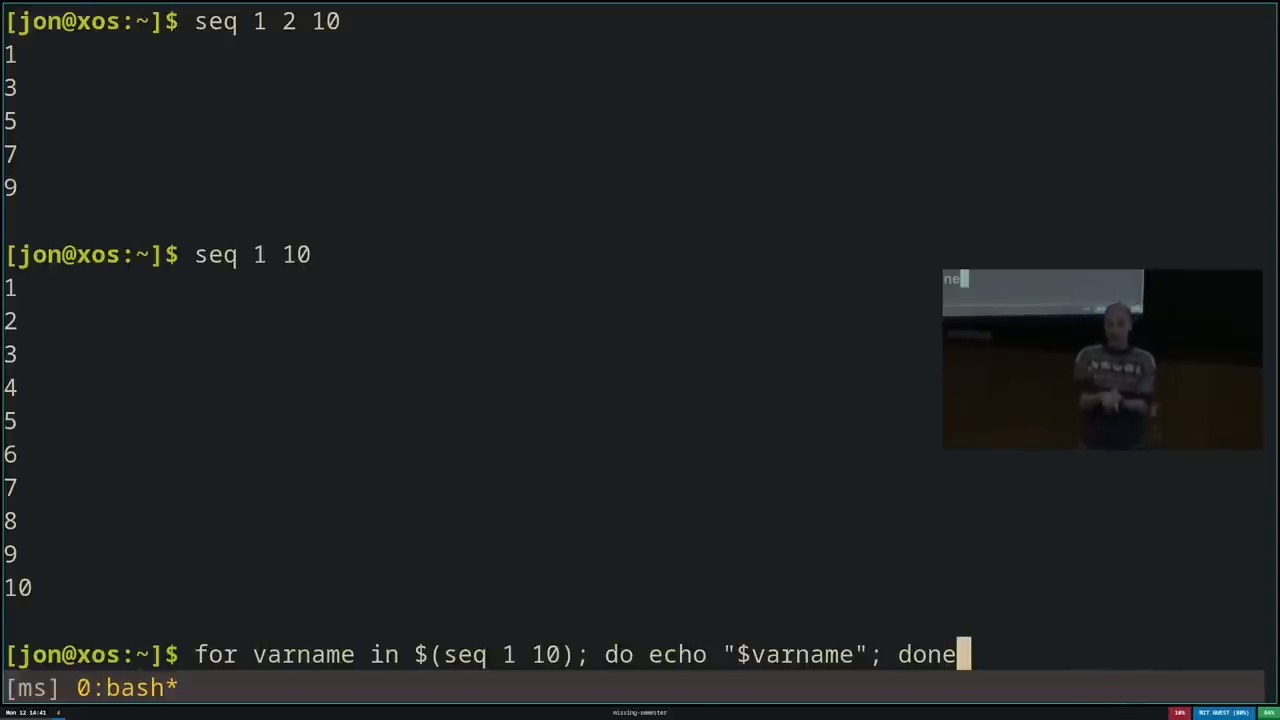
\includegraphics[width=0.92\textwidth]{figures/fig_25_for_seq.jpg}
\caption{\texttt{for} 循环配合 \texttt{\$(seq 1 10)} 迭代数字\vtag}
\end{figure}
\srcnote{01:05:00--01:05:15}
\end{minipage}


\texttt{for} 循环形如 \texttt{for varname in a b c d; do echo "\$varname"; done}，依次把变量设为 a、b、c、d。如果想要熟悉的按数字迭代的循环，可以用一个小技巧：\texttt{\$(...)} 是 bash 里“运行括号里的程序，然后用它的输出替换整个表达式”的写法，称为命令替换。\texttt{seq 1 10} 打印 1 到 10 的数字，所以 \texttt{for i in \$(seq 1 10)} 就是循环 10 次。讲者解释，这不能完全代替管道，因为命令替换把输出变成了参数，而例如 \texttt{sort} 是从输入读取内容来排序，并不排序它的参数。

\begin{lstlisting}[language=bash]
if grep 2026 thedate.txt; then echo "it's 2026"; fi
while grep 2026 thedate.txt; do echo "it's still 2026"; sleep 10; done
for i in $(seq 1 10); do echo "$i"; done
\end{lstlisting}

\subsection{test 与方括号}

\noindent\begin{minipage}{\textwidth}
\begin{figure}[H]
\centering
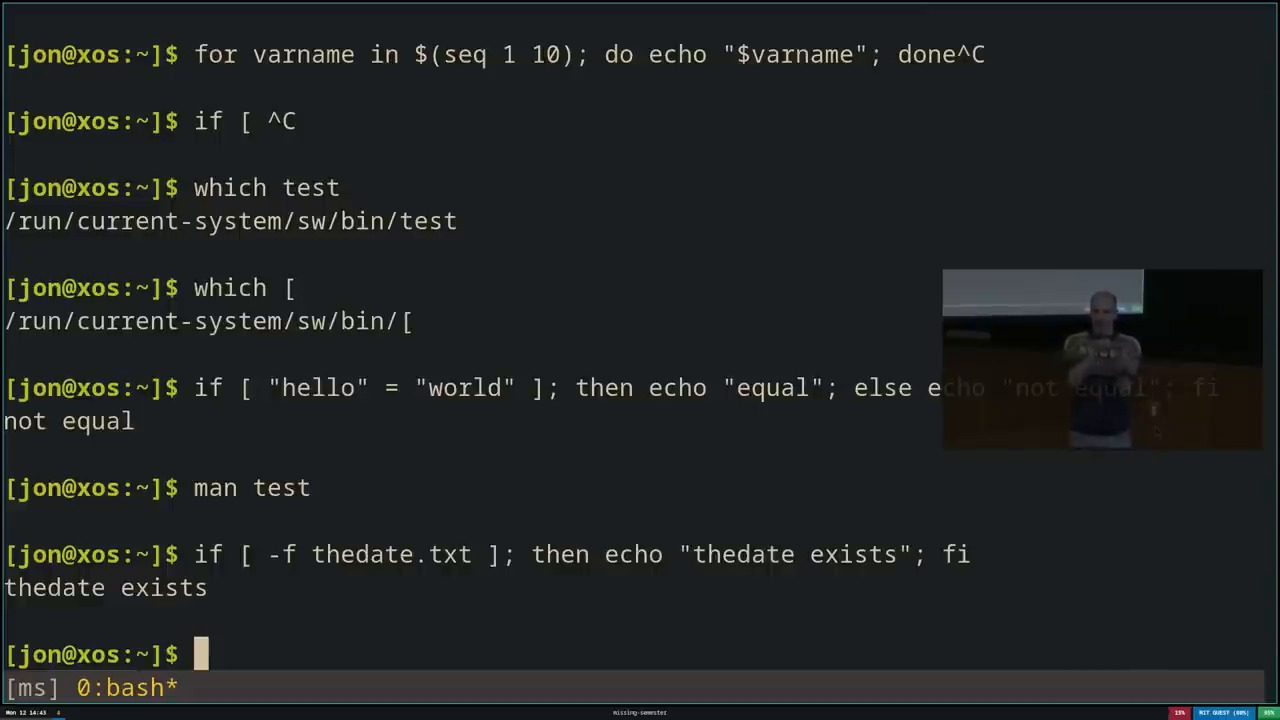
\includegraphics[width=0.92\textwidth]{figures/fig_26_test.jpg}
\caption{\texttt{which [} 与 \texttt{which test} 指向同一类程序，\texttt{[ -f thedate.txt ]} 判断文件是否存在\vtag}
\end{figure}
\srcnote{01:07:00--01:07:15}
\end{minipage}


讲者运行 \texttt{which test} 和 \texttt{which [}，发现它们是同一个程序，方括号只是更简短的写法。可以把它当作 \texttt{if} 的条件来运行，它的约定是条件为真时退出码为 $0$。例如 \texttt{if [ "hello" = "world" ]; then echo equal; else echo not equal; fi} 会打印 not equal。\texttt{-f} 参数测试是否存在以后面参数命名的文件。借助这些，就能构造相当复杂的自动化流程。

有同学问：既然 \texttt{if} 能工作是因为有一个做比较的程序，那 \texttt{if} 本身也是程序吗？讲者说这是个好问题：\texttt{if} 不是程序，而是 Shell 语言的关键字。又有同学问屏幕上的 \texttt{\^{}C} 是做什么的：那只是按下 Ctrl+C 退出当前命令时终端打印出来的符号，本身不做任何事。讲者还提到，读 bash 代码时经常看到双方括号 \texttt{[[ ]]}，那是 bash 内置的、更安全的 \texttt{test} 形式，在引号处理等方面的怪异行为更少。

\begin{warningbox}{方括号两侧必须有空格}
讲义作者提醒：既然 \texttt{[} 是一个程序名，\texttt{]} 是它的最后一个参数，那么 \texttt{[ -f file ]} 里的空格一个都不能少；写成 \texttt{[-f file]} 时，Shell 会去找一个叫 \texttt{[-f} 的程序。比较字符串时也要给变量加引号，写成 \texttt{[ "\$var" = "string" ]}。
\end{warningbox}

\subsection{本章小结}

管道和重定向决定数据从哪里来、到哪里去；\texttt{if} 和 \texttt{while} 依据命令的退出码工作，\texttt{test} 和 \texttt{[} 是专门用来产生退出码的程序；\texttt{\$(...)} 把命令输出变成参数。最后一步，是把这些命令写进一个文件。

\section{Shell 脚本}

\subsection{一个复现偶发失败测试的脚本}

\noindent\begin{minipage}{\textwidth}
\begin{figure}[H]
\centering
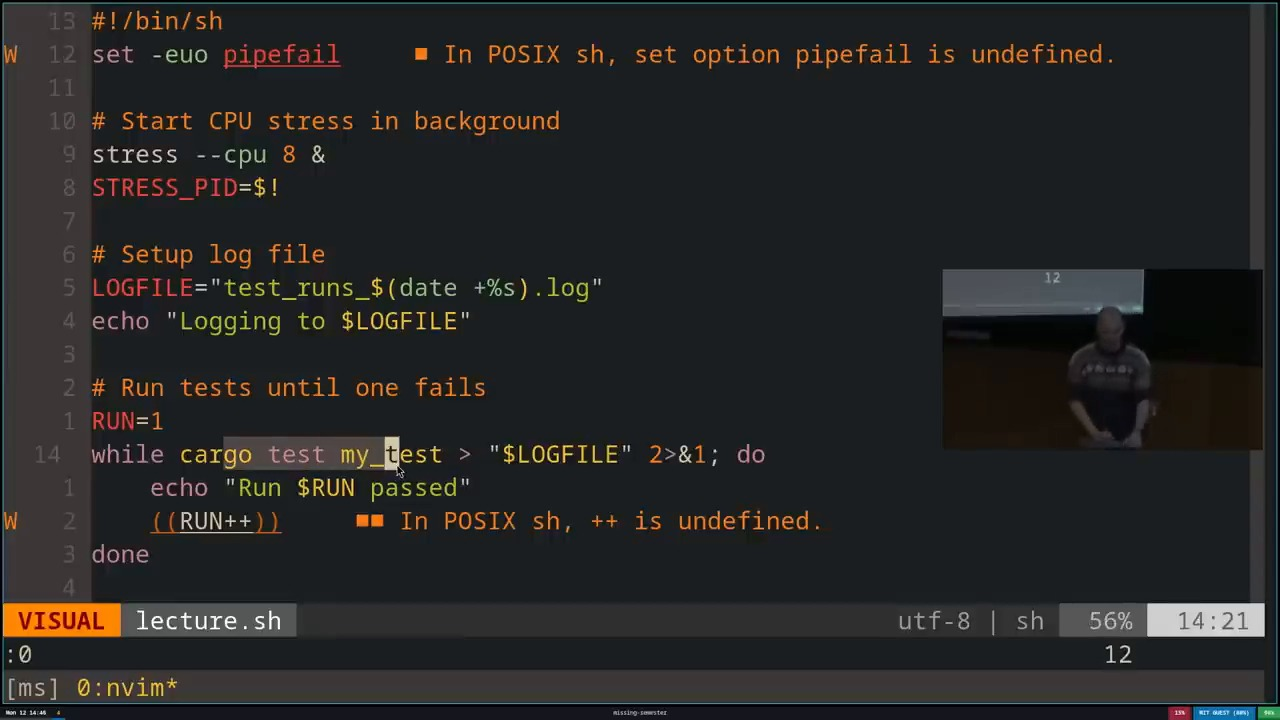
\includegraphics[width=0.92\textwidth]{figures/fig_27_script.jpg}
\caption{讲义中的示例脚本：在后台施加 CPU 压力，同时循环运行测试直到失败\vtag}
\end{figure}
\srcnote{01:09:30--01:09:45}
\end{minipage}


讲者说，在提示符里可以写很长的 Shell 程序，但通常更推荐写进 \texttt{.sh} 文件。bash 执行一个程序时，会从上到下逐行运行，就像你在提示符里一行行输入一样，语言完全相同。讲义里的这个脚本会在循环中不断运行某个测试直到它失败，只打印失败那次的输出，同时在后台对 CPU 施加压力。他说这在复现偶尔失败的测试时非常有用：比如某个测试每 $100$ 次运行才失败一次，与其自己坐在那里按上箭头、回车、上箭头、回车，不如运行一次这个脚本，去喝杯咖啡，回来时磁盘上就有一个文件保存着失败那次测试的输出。

\begin{lstlisting}[language=bash]
#!/bin/bash
set -euo pipefail

# Start CPU stress in background
stress --cpu 8 &
STRESS_PID=$!

# Setup log file
LOGFILE="test_runs_$(date +%s).log"
echo "Logging to $LOGFILE"

# Run tests until one fails
RUN=1
while cargo test my_test > "$LOGFILE" 2>&1; do
    echo "Run $RUN passed"
    ((RUN++))
done

# Cleanup and report
kill $STRESS_PID
echo "Test failed on run $RUN"
echo "Last 20 lines of output:"
tail -n 20 "$LOGFILE"
echo "Full log: $LOGFILE"
\end{lstlisting}

\subsection{shebang 与严格模式}

脚本的第一行以井号和感叹号开头，叫 shebang（hash bang）。讲者解释，它告诉系统用哪个程序来执行这个文件：直接运行 \texttt{./lecture.sh}，等价于运行 \texttt{/bin/sh}、并把 \texttt{lecture.sh} 作为输入。shebang 的妙处在于它不一定是 bash：在他的系统上 \texttt{/bin/sh} 就是 bash，但同样可以写 \texttt{/usr/bin/python}，然后在这个文件里写 Python 代码。有同学问能否用于需要编译的语言：讲者说只要有一个包装程序能编译并运行它，就能这样用。

第二行让 bash 以更严格的模式运行，能避免 Shell 脚本中许多常见的陷阱。按课程讲义的说明：\texttt{-e} 表示任何命令失败时脚本立即退出；\texttt{-u} 表示使用未定义的变量时报错，而不是默默当作空字符串；\texttt{-o pipefail} 表示管道中只要有程序失败，整个脚本也会尽早退出。

\begin{warningbox}{\texttt{/bin/sh} 不一定是 bash}
讲者的编辑器在这个脚本上标出了一条提示：在 POSIX sh 中，\texttt{set -o pipefail} 是未定义的，\texttt{((RUN++))} 这样的算术写法也是。讲义作者提醒：讲者的系统上 \texttt{/bin/sh} 恰好是 bash，但在 Debian、Ubuntu 上它是 dash，这些写法会出错。用到 bash 特性的脚本，shebang 应写成 \texttt{\#!/bin/bash} 或 \texttt{\#!/usr/bin/env bash}。
\end{warningbox}

\subsection{执行权限}

\noindent\begin{minipage}{\textwidth}
\begin{figure}[H]
\centering
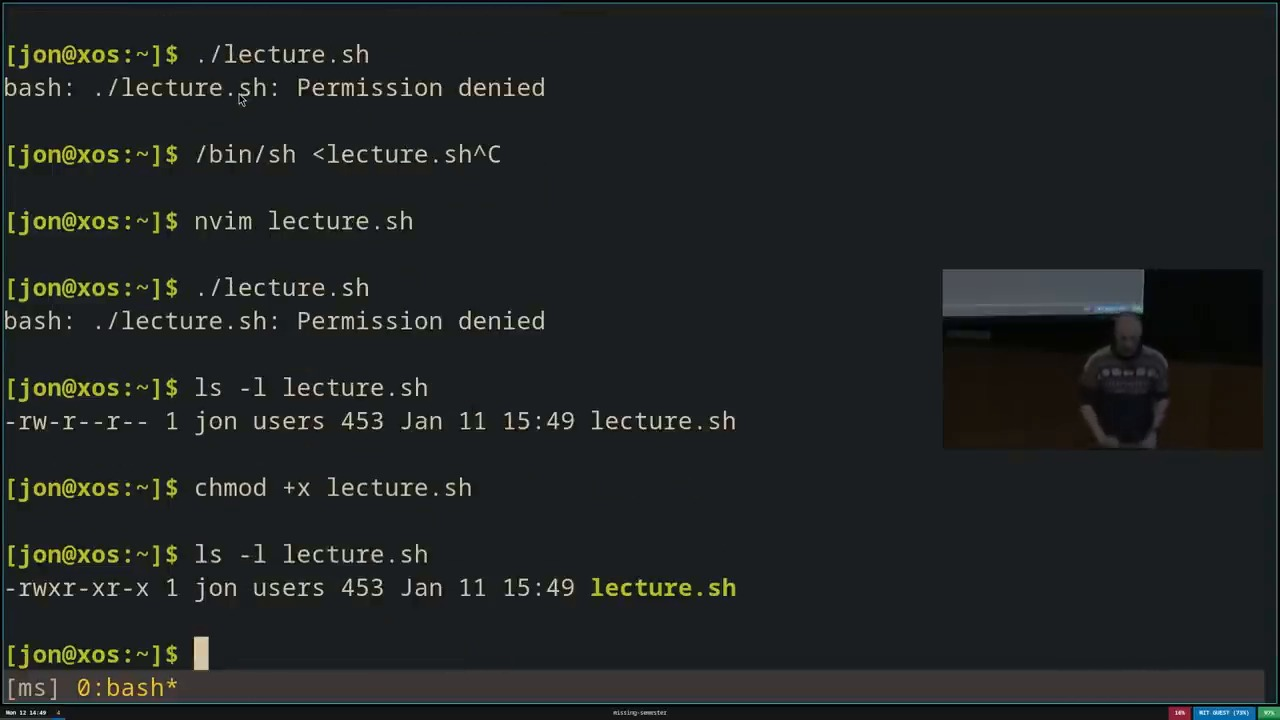
\includegraphics[width=0.92\textwidth]{figures/fig_28_chmod.jpg}
\caption{\texttt{chmod +x} 之后，\texttt{ls -l} 显示出执行位，脚本才能直接运行\vtag}
\end{figure}
\srcnote{01:13:00--01:13:15}
\end{minipage}


讲者最初运行脚本时被拒绝了，提示 permission denied。这是因为运行可执行文件时，Shell 会检查你对这个文件是否有执行权限。\texttt{ls -l} 显示了更多信息，其中包括权限位；执行 \texttt{chmod +x lecture.sh} 添加执行权限后再 \texttt{ls}，文件名换了颜色，因为 \texttt{ls} 会给可执行文件着色，现在有了执行位。再运行 \texttt{./lecture.sh}，它确实运行了，并抱怨找不到 Rust 的安装，因为这只是一个示例脚本。

\begin{practicebox}{读懂 \texttt{ls -l} 的权限位}
讲义作者整理：\texttt{-rwxr-xr-x} 第一个字符表示类型（\texttt{-} 为普通文件，\texttt{d} 为目录），之后每三位一组，依次是所有者、所属组、其他人的读（r）、写（w）、执行（x）权限。\texttt{chmod +x} 为所有人加上执行权限，\texttt{chmod u+x} 只为所有者添加。
\end{practicebox}

\subsection{本章小结}

Shell 脚本就是写进文件的命令序列，shebang 决定由谁来解释，\texttt{set -euo pipefail} 让错误不再被悄悄忽略，执行权限决定文件能否直接运行。

\section{总结}

讲者以推荐习题结束了这一讲：讲义里有更多细节和其他有用的程序，强烈建议大家去看、去做习题。回顾这一讲：
\begin{itemize}
\item 这门课教的是课程之外“默认你会”的工具，重在让你知道有哪些可能，再自己深入；
\item 终端是窗口，Shell 是解释命令的程序，bash 与 zsh 是本课的基准；
\item 命令按空白切分为程序和参数，引号与反斜杠控制切分；\texttt{man} 与 \texttt{-{}-help} 是第一手文档；
\item 绝对路径、相对路径、\texttt{.}、\texttt{..}、\textasciitilde{} 用于在文件系统中移动；Shell 按 \texttt{PATH} 找程序；
\item \texttt{grep}、\texttt{sed}、\texttt{find}、\texttt{awk} 等小程序通过管道组合，可以一条命令完成复杂分析；
\item Shell 是一门编程语言，有重定向、条件、循环和命令替换，可以写成带 shebang 的脚本。
\end{itemize}

\begin{practicebox}{自测}
\begin{enumerate}
\item 为什么 \texttt{echo hello      world} 和 \texttt{echo "hello      world"} 输出不同？
\item 用 \texttt{which -a} 找出你系统里有多个副本的一个程序，Shell 会运行哪一个？
\item 写一个命令，找出主目录下所有大于 100M 的文件并按大小显示。
\item 逐段运行 SSH 日志那条管道（可换成本机任意日志），说出每一步之后数据的样子。
\item 写一个脚本，循环运行一个随机失败的命令直到它失败，并报告运行了多少次。
\end{enumerate}
\end{practicebox}

\end{document}
